\documentclass[12pt]{report}
\usepackage[utf8]{inputenc}
\usepackage{graphicx}
\graphicspath{ {./images/} }

%margins
\usepackage{geometry}
 \geometry{
 a4paper,
 margin=3cm
 }

\usepackage{amsmath}
\usepackage{fancyhdr}
\usepackage[square,sort,comma,numbers]{natbib}
\usepackage{amsfonts}

\usepackage{booktabs}
\usepackage{multicol}
\usepackage{multirow}
\usepackage{subcaption}
\usepackage{hyperref}
\hypersetup{}
\urlstyle{same}

% chapter titles
\usepackage{titlesec}
\titleformat{\chapter}[hang] 
{\normalfont\huge\bfseries}{\thechapter}{1em}{} 

% paragraph titles1
\titleformat{\paragraph}{\normalfont\normalsize\bfseries}{\theparagraph}{}{}
\titlespacing*{\paragraph}
{0pt}{3.25ex plus 1ex minus .2ex}{1.5ex plus .2ex}
\setlength{\parskip}{1em}

% chapter pages numbering
\fancypagestyle{plain}{%
  \renewcommand{\headrulewidth}{0pt}%
  \fancyhf{}%
  \rhead{ \thepage}
}

% line breaking
\widowpenalties 1 1000000
\raggedbottom


\begin{document}

\begin{titlepage}
    \begin{center}
        
\includegraphics[width=0.4\textwidth]{HTW_logo}    
    
        \vspace*{1cm}
        
        \Large
        \textbf{Implementation and Evaluation of \\ Image Synthesis Methods for Improving Image Retrieval}
        
        \Large
        \vspace{0.5cm}
        Master Thesis\\
        
        \vspace{1cm}
        \normalsize
        presented for the degree of\\
        \textbf{Master of Science (M.Sc.)} by
        
        \vspace{1cm}
		\large
        Sona Pecenakova
        
        \vspace{1.5cm}
        
\vfill
\noindent    
University of Applied Sciences Berlin\\
Faculty 4: School of Computing, Communication and Business\\
Study Programme: International Media and Computing

    \end{center}
        
\vspace{0.8cm}

\noindent
October 2018, Berlin \\
\noindent
1. Supervisor: Prof. Dr.-Ing. Kai Uwe Barthel\\
2. Supervisor: M.Sc. Nico Hezel\\
     
     
\end{titlepage}

\pagestyle{plain}
\pagenumbering{gobble}
\renewcommand{\baselinestretch}{0.75}\normalsize
\tableofcontents
\renewcommand{\baselinestretch}{1.0}\normalsize
\clearpage

% ==============================================================
% Introduction
% ==============================================================

% page numbering
\pagestyle{fancy}
\fancyhf{}
\renewcommand{\chaptermark}[1]{\markboth{\thechapter.\space#1}{}} 
\lhead{\slshape\nouppercase{\leftmark}}
\rhead{ \thepage}
\renewcommand{\headrulewidth}{.5pt}
\pagenumbering{arabic}
\chapter{Introduction}

\section{Motivation}
% Motivation
According to Yann LeCun, a machine learning pioneer, generative adversarial models are one of the most relevant recent developments in deep learning \cite{yann_lecun_what_2016}. Introduced in 2014, these models opened countless possibilities of generating realistic new content by making two neural networks compete with each other. In the past few years, researchers have developed various adversarial implementations that can generate, for example, a Monet painting from a photograph or  a high-resolution fake celebrity face.

One field of computer vision that can benefit from the application of generative models is image retrieval. Most of currently available image retrieval systems rely on machine learning algorithms to extract relevant image descriptors, which are then be compared to retrieve images with similar content. The question is whether the retrieval can benefit from new synthesized content by applying generative adversarial models.

A suitable area to evaluate this hypothesis is online fashion retail. Not only due to the vast amount of visual, as well as textual content available, but also because choice of fashion products is subjective. Navigating through all alternatives to find a product that fits the requirements of an individual is time-consuming, and also highly dependent on the filtering and search options that a given website offers. Retrieving relevant and customized products can therefore help speed up the search process.

% Something like current research has already focused on generating new fashion items that could then be produced, or 3D printed. However, this type of synthesis does not have much practical use. Using hte generated images to retrieve existing products that can be bought on the other hand, can find practical use in fashion retail stores or aggregator sites.

\section{Objective}
The goal of this thesis is to evaluate existing generative models for user-driven modification of fashion images, and implement a system that enables the user to influence the retrieval of similar products. Hereby, the main goal of the synthesis is not to generate highly realistic output, but output realistic enough to improve the retrieval of similar images. To analyze the possibilities of user-driven modification, several image-to-image translation models are compared and experimented on a dataset consisting of fashion products. The experiments further analyze various features that can be used to retrieve similar images from the dataset.


\section{Thesis Structure}
The following chapter describes the background of the two main topics of this thesis: generative adversarial networks and content-based image retrieval systems. The third chapter introduces some of the existing fashion datasets, and the fashion dataset used for the experiments. It also introduces several generative adversarial models for image-to-image translation and their main characteristics. Furthermore, it also introduces several image descriptors that can be used to retrieve similar images. Chapter four documents the experiments with the evaluated image-to-image translation networks and retrieval features. The results and the final application are then summarized in chapter five, as well as possible causes of synthesis issues that occured in some of the experiments. The last chapter concludes the work and presents possibilities of future development of the project.

\newpage
% ==============================================================
% GANS
% ==============================================================
\chapter{Background}
This chapter introduces the background of the two building blocks of this thesis: generative adversarial networks (GAN) and content-based image retrieval systems (CBIR). It describes GAN architecture, training objective and some of the instabilities that commonly occur when training a GAN model. It also mentions some specific architectures that are used throughout this thesis. The second part of this chapter introduces content-based image retrieval systems, the way they had been implemented in the past and how they changed since the rise of the convolutional neural networks.

% ==============================================================
% ==============================================================
\section{Generative Adversarial Networks}
% ==============================================================

Introduced in 2014 \cite{goodfellow_generative_2014}, generative adversarial  networks, so-called GANs, have been the focus of countless research papers and creative implementations. GANs have learned how to generate an image of a cat from a simple drawing \cite{hesse_image--image_nodate}, create new artworks \cite{rkjones4_gangogh_2018}, generate high-resolution celebrity faces \cite{karras_progressive_2017}, colorize grayscale images and much more.

\begin{figure}[b]
\centering
{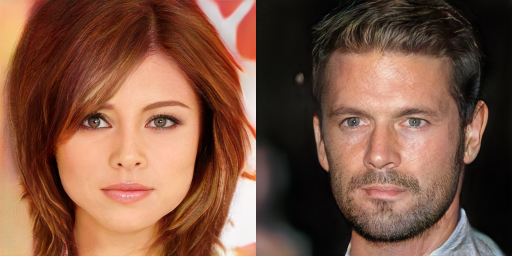
\includegraphics[width=\linewidth]{02_background/gan_faces}}
\caption{\label{fig:mnist} \textbf{Generated celebrity faces.} Figure reprinted from \cite{karras_progressive_2017}.}
\end{figure}

To generate new realistic samples, two neural networks are trained to compete with each other. Each network is trying to get better at its own task while trying to prevent the other network from doing so. 

A common analogy can be found in money forgery: while a fraud investigator is trying to detect real bills from fraudulent ones, the money forger is trying to improve his falsification techniques, so that the investigator is unable to tell the difference.

In computational world, the investigator is a neural network called \textit{Discriminator} competing with the forger network called \textit{Generator}. The discriminator is trained to classify samples from the original dataset as ,,real'', and samples generated by the generator as ,,fake''. The generator is trained to fool the discriminator, so that it cannot correctly classify generated samples as fake.

Figure \ref{fig:mnist} shows example data points of the hand-written digits dataset MNIST \cite{lecun_mnist_nodate}, along with samples generated with a deep convolutional GAN \cite{kim_dcgan-tensorflow_2018} - the samples from the original and generated distributions are almost indistinguishable.

\begin{figure}[h]
\centering
\subcaptionbox{Original MNIST}
{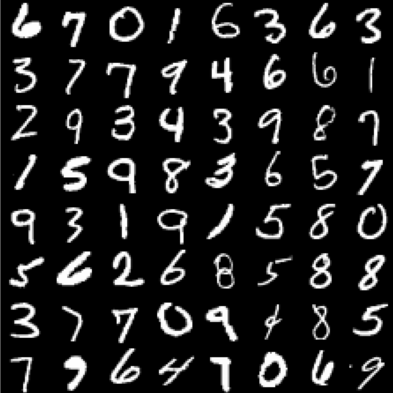
\includegraphics[width=.35\linewidth]{02_background/mnist_orig}}\hspace{0.5cm}
\subcaptionbox{Generated MNIST}
{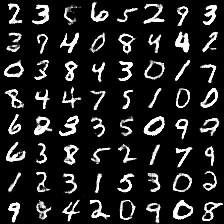
\includegraphics[width=.35\linewidth]{02_background/mnist_dcgan}}
\caption{\label{fig:mnist} \textbf{MNIST Example.}
(a) Sample from the original MNIST dataset \cite{lecun_mnist_nodate}. (b) Samples generated with a GAN \cite{kim_dcgan-tensorflow_2018}.}
\end{figure}

% ==============================================================
\subsection{Architecture}
% ==============================================================

Figure \ref{fig:gan} illustrates a typical GAN architecture. The discriminator is a common Convolutional Neural Network \cite{lecun_convolutional_1995}, which takes an image as input and trains to extract necessary information from the input in order to classify the image. The output is a scalar value, classifying the image as real, coming from the dataset, or fake, coming from the generator.

\begin{figure}[h]
\centering
{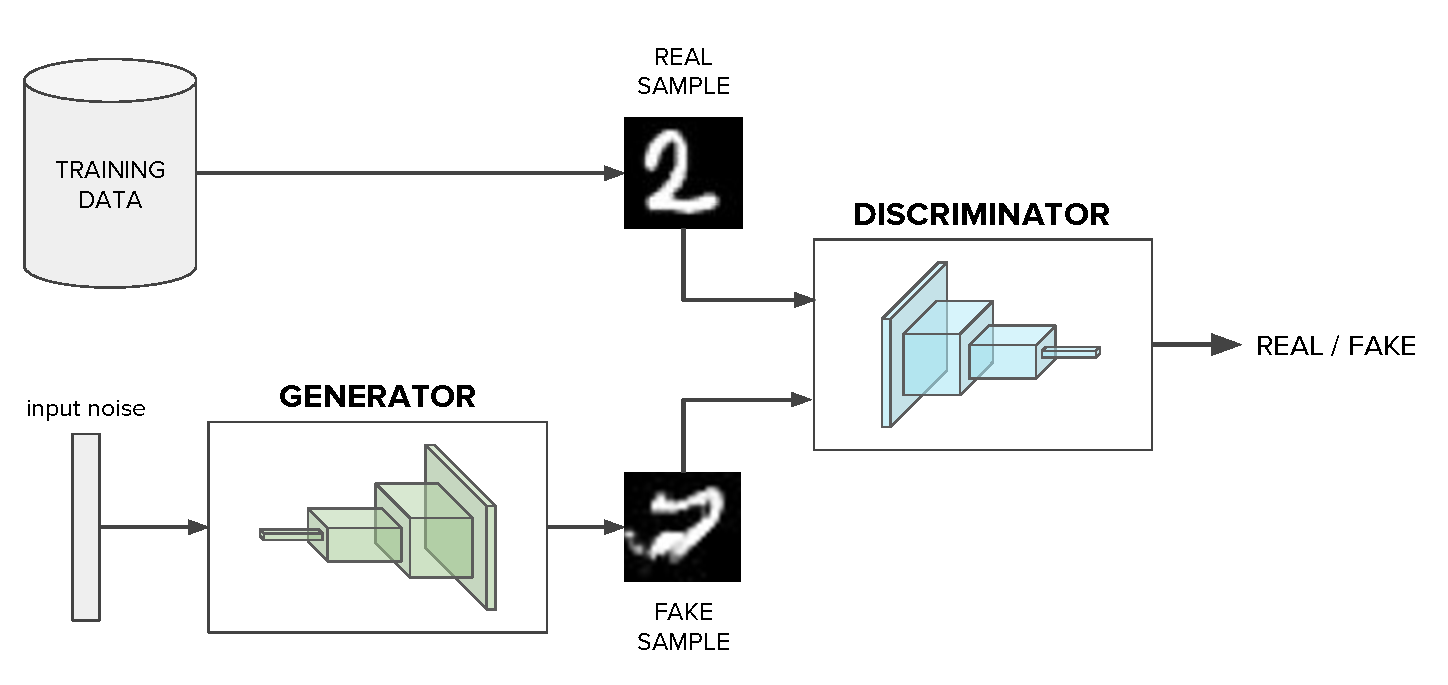
\includegraphics[width=\linewidth]{02_background/gan_model}}
\caption{\label{fig:gan} \textbf{GAN model.} The generator network produces fake images, which the discriminator network tries to distinguish from the real samples coming from the dataset.}
\end{figure}

The generator architecture is similar, however it uses a transposed convolution, the so-called ,,deconvolution'', to produce a 3-dimensional output from a 1-dimensional input vector. The generator input vector is sampled randomly.

The discriminator receives either a sample from the real data distribution, or a generated sample. The classification output of the discriminator is back-propagated  through the discriminator, as well as the generator network, in order to adjust the networks weights to improve the training objective.

% ==============================================================
\subsection{Training Objective} \label{sec:GAN_training}
% ==============================================================

Given input data with distribution $p(x)$, the generator $G$ is a neural network, that maps random input noise $z$ to the input space, as $G(z, \theta_{g})$, learning the model distribution $\hat{p}(x)$. The discriminator $D$ is a second neural network $D(x, \theta_{d})$ with a single scalar output, classifying the input $x$ as real, sampled from data distribution $p(x)$, or as fake, sampled from the model distribution $\hat{p}(x)$. 

The training objective of the discriminator is to maximize the probability of assigning the correct label, while the objective of the generator is to minimize this probability. The loss function of the GAN can be described as the minimax objective,
\begin{equation}
\underset{G}{\mathrm{min}} \ \underset{D}{\mathrm{max}} \ \mathcal{L}(D,G) = \mathbb{E}_{x \sim p_{data}(x)}[\log D(x)] + \mathbb{E}_{z \sim p_{z}(z)}[\log (1 - D(G(z))].
\label{eq:minimax}
\end{equation}

The gradient of this loss function is back-propagated through the networks in respect to each of the network parameters, $\theta_{d}$ and $\theta_{g}$, followed by a parameter update using an optimization algorithm such as gradient descent.

% ==============================================================
\subsection{Training Challenges} \label{sec:gan_diff}

In theory, the minimax game described in equation \ref{eq:minimax} is played until generator has perfectly modeled the distribution $p(x)$, so that discriminator classifies the authenticity of the samples at random. In reality, the training of a GAN can prove to be unstable and finding the right balance between the two networks is difficult.

It can happen, for example, that the gradient descent gets stuck in a cycle, where a modification to the discriminator weights reduces the discriminator loss and increases the generator loss, while the following modification of generator weights does the opposite \cite{salimans_improved_2016}. In this scenario, the gradient descent is not able to converge.

One of the common causes of instability is the vanishing gradient problem: when the discriminator gets confident at classifying the generated samples as fake early on, the generator gradient vanishes and the generator has no opportunity to improve. 

In the seminal GAN paper, Goodfellow et al. \cite{goodfellow_generative_2014} suggest $G$ to be trained to maximize $\mathbb{E}_{z \sim p_{z}(z)}[\log D(G(z))]$, instead of minimizing the original term $\mathbb{E}_{z \sim p_{z}(z)}[\log (1 - D(G(z))]$ used in Equation \ref{eq:minimax}, to avoid vanishing gradients. 

Since then, other research on how to stabilize GAN training has been published \cite{arjovsky_towards_2017}\cite{roth_stabilizing_2017}\cite{salimans_improved_2016}. The recommended techniques to prevent the vanishing gradient problem are mostly focused on confusing the discriminator, to give the generator an advantage in the training. 

One of the techniques that can be applied is to add noise to the labels that define whether the image is real (1.0) or fake (0.0). As shown by Saliman et al. \cite{salimans_improved_2016}, varying the labels with a slight noise can help to stabilize the training. To further confuse the discriminator, we can also occassionally flip the labels. 

% ==============================================================
% Deep Convolutional GANs
% ==============================================================
\subsection{Deep Convolutional GANs} \label{sec:dcgan}


Many GAN implementations base their network architecture on Deep Convolutional GANs (DCGAN), described by Radford et al. \cite{radford_unsupervised_2015}. The authors introduced architectural guidelines for convolutional networks used in GANs, that stabilize the training and result in more realistic outputs.

\begin{figure}[t]
\centering
{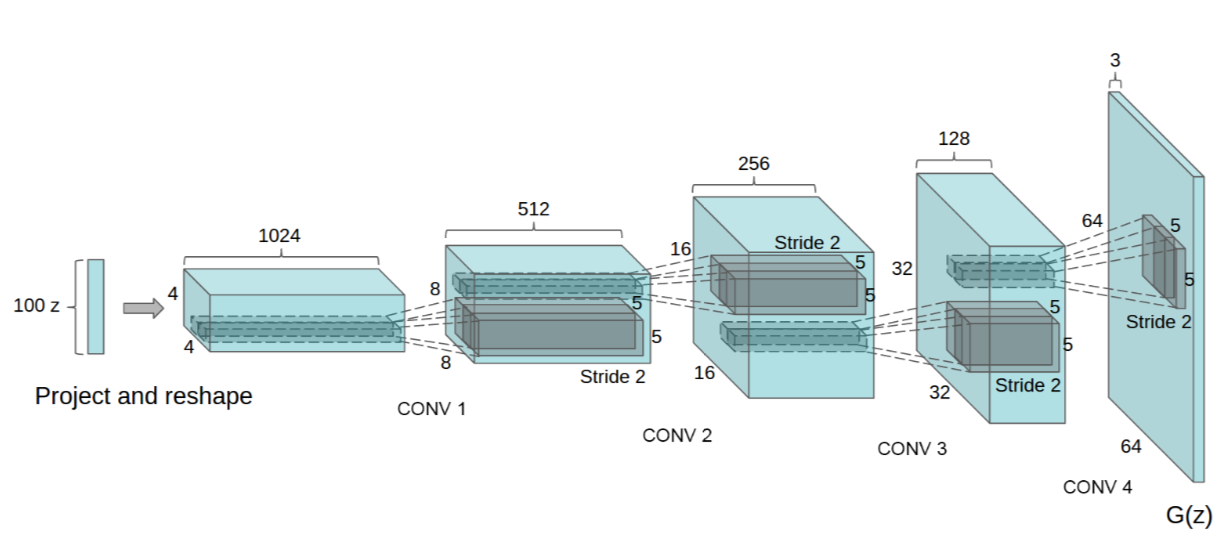
\includegraphics[width=\linewidth]{02_background/dcgan_generator}}
\caption{\label{fig:dcgan} \textbf{DCGAN Generator.} An example architecture of a DCGAN generator $G(z)$. The random input noise $z$ is mapped to a 64x64 image with 3 color channels via fractionally-strided convolution layers. Figure reprinted from \cite{radford_unsupervised_2015}.}
\end{figure}

After experimenting with CNN architectures commonly used in computer vision tasks, Radford et al. \cite{radford_unsupervised_2015} have found that this set of architecture modifications has a positive effect on the stability and convergence speed of the models:
\begin{itemize}
\item \textbf{All Convolutional Net}: A common practice in convolutional neural networks are \textit{Pooling Layers}, which reduce the number of parameters by filtering the convolution outputs, taking maximum or average of a given region. However, the authors have found that using an All Convolutional Network \cite{springenberg_striving_2014}, which replaces all pooling layers with a strided convolution, leads to more stable results.
\item \textbf{Fully-Connected Layers}: The authors argue \cite{radford_unsupervised_2015}, that avoiding fully-connected layers deeper in the network stabilizes the network. They keep fully-connected layers only in the discriminator output layer and generator input layer, as they found that removing all fully-connected layers would slow down the convergence.
\item \textbf{Batch Normalization}: Batch Normalization \cite{ioffe_batch_2015} has been introduced in common image-classification to make models more robust to parameter initialization and speed up training. The DCGAN paper shows that including a batch-norm layer in all GAN layers (except discriminator output and generator input), helps generators start learning and produce diverse outputs.
\item \textbf{Activation Functions}: As opposed to maxout activation suggested by the original GAN paper \cite{goodfellow_generative_2014}, GANs seem to benefit from \textit{Leaky ReLU} activation function in discriminator, and \textit{ReLU} activation function for generator, except last generator layer, which uses a \textit{tanh} activation function.
\end{itemize}

The DCGAN architecture has been established as the state-of-the-art architecture and is the model for most of the GAN implementations mentioned in this thesis.

% ==============================================================
% Conditional GANs
% ==============================================================
\subsection{Conditional GANs} \label{sec:cond_gan}
Mirza and Osindero \cite{mirza_conditional_2014} introduced the Conditional Generative Adversarial Networks to influence the output of a GAN. By conditioning both the discriminator and the generator on additional information, the generator learns to output realistic samples based on given input.

\begin{figure}[t]
\centering
{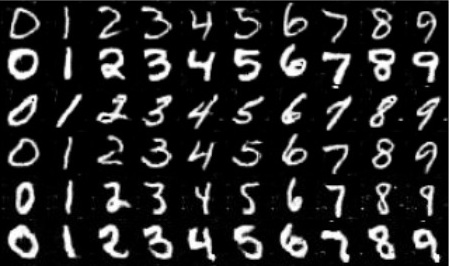
\includegraphics[width=.6\linewidth]{02_background/mnist_cgan2}}
\caption{\label{fig:cgan} \textbf{MNIST digits genereated with Conditional Adversarial Networks.} Each row is conditioned on one label. Figure reprinted from \cite{mirza_conditional_2014}.}
\end{figure}

Considering the previous example of MNIST hand-written digits synthesis, one can condition the networks using the digits as class labels, and control the network to generate an image of a specific digit. There have also been experiments with text-to-image translation \cite{reed_generative_2016}, where the network is conditioned on a text description of an image, and various image-to-image translation GANs \cite{yoo_pixel-level_2016}\cite{yoo_pixel-level_2016}\cite{pathak_context_2016}.

The training objective of conditional GAN is following:
\begin{equation}
\underset{G}{\mathrm{min}} \ \underset{D}{\mathrm{max}} \ V(D,G) = \mathbb{E}_{x \sim p_{data}(x)}[\log D(x|c)] + \mathbb{E}_{z \sim p_{z}(z)}[\log 1 - D(G(z|c))].
\label{eq:cgan}
\end{equation}

The conditioning information $c$, such as a class label, text, or another image, is fed to both discriminator $D$ and generator $G$ as additional input layers.


% ==============================================================
% Image Retrieval
% ==============================================================
\section{Content-Based Image Retrieval}
The idea of content-based image retrieval systems (CBIR) is to find semantically similar images without depending on textual meta-data, such as tags or descriptions. Instead these systems only rely on the pixel values and try to find similarities based on visual features that can be extracted from the content of the images.

CBIR is a field of computer vision that has seen a lot of changes since the rise of fast and available deep learning algorithms. While the first CBIR implementations have relied on low-level features such as color and texture to identify similar images, today the state-of-art techniques rely on high-dimensional descriptors produced by convolutional neural networks.

The systems are used for many specific applications in different fields, e.g: medicine, retail or archives. Many CBIR systems are also freely available online, such as the visual image search on Google, or a tool for exploring large amounts of images based on their similarities called \textit{PicsBuffet} \cite{mackowiak_picsbuffet_nodate}.


\begin{figure}[h]
\centering
{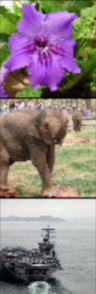
\includegraphics[height=6cm]{02_background/CBIR/cnn_cbir_input}}
{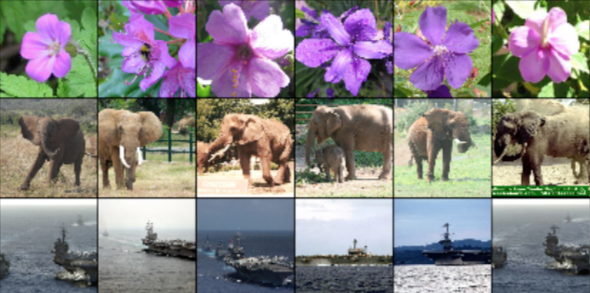
\includegraphics[height=6cm]{02_background/CBIR/cnn_cbir_retrieval}}
\caption{\label{fig:conv_cbir} \textbf{Image Retrieval with CNN Features}. Images in the left column are compared to images from a training set to find most similar matches. The images are compared based on 4028-dimensional feature vectors extracted from the last hidden layer of a convolutional neural network. Figure reprinted from \cite{NIPS2012_4824}.}
\end{figure}

\pagebreak
\subsection{Low-Level Visual Features}
The implementations of CBIR systems that do not use deep learning algorithms are mostly based on low-level features. Feature that describe the color, texture or shapes in the image are usually combined together to to create image descriptors that can be compared to retrieve the most similar images.

\subsubsection{Color Features}
Color is one of the most basic features of an image. While there are many possibilities to describe the color of an image, such as average color or selecting a few dominant colors, the color histogram has proven to be a robust choice and is often used as a baseline when comparing other color features \cite{Torres_content-basedimage}.

To create a color histogram, the occurence of each color, as described by the image color space such as RGB, is counted. These counts can then be grouped into bins and represented as relative frequencies \cite{Swain1991}.

\begin{figure}[h]
\centering
\subcaptionbox{RGB Image}{\includegraphics[height=5cm]{02_background/CBIR/atacama}}
\subcaptionbox{3D Color Histogram}{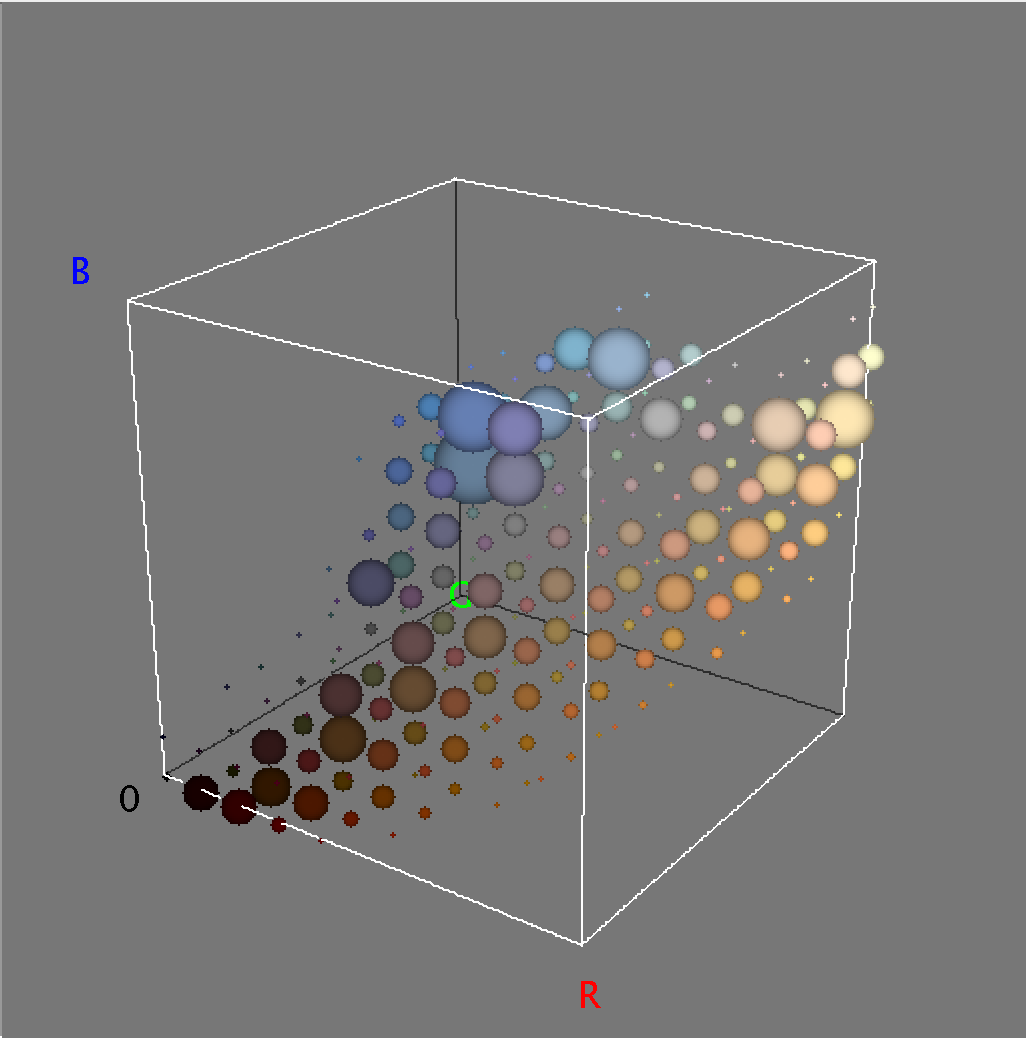
\includegraphics[height=5cm]{02_background/CBIR/color_hist}}
\caption{\label{fig:color_hist} \textbf{Color Histogram}. A 3-D visualization of the color histogram with 200 color bins for an RGB image. Histogram visualization created with 3D Color Inspector \cite{barthel_3d_nodate}.}
\end{figure}

The main advantage of color features is that they are invariant to image transformations such as rotation. However, founding the retrieval only on colors is insufficient, since images that share similar color histograms do not necessarily display the same content and images showing the same content can have different color palettes.

\subsubsection{Texture Features}
Although texture feature can be perceived equally important to color feature, it is more difficult to define texture. There are several methods for extracting texture that can be based on statistics, such as the co-occurence matrix, human perception, such as Tamura features, or signal processing, such as Gabor filters or Fourier transformations.

Figure \ref{fig:texture_feat} shows examples of textures with their respective Tamura texture descriptors \cite{tamura1978textural}. They use six terms to describe a given texture: coarseness, contrast, directionality, line-likeness, regularity and roughness. 

\begin{figure}[h]
\centering
{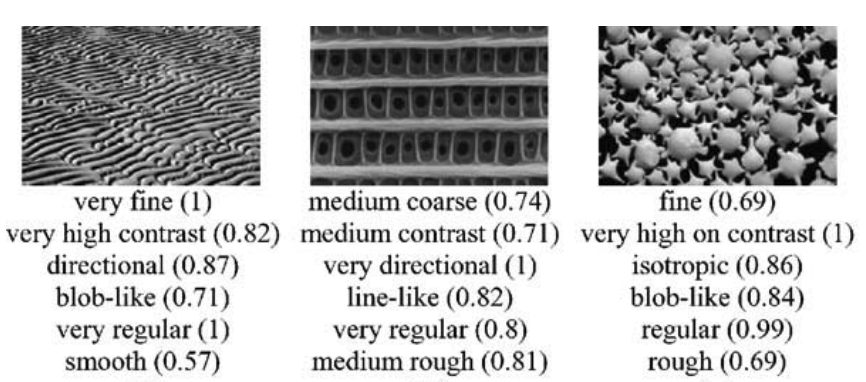
\includegraphics[width=0.7\linewidth]{02_background/CBIR/texture_features}}
\caption{\label{fig:texture_feat} \textbf{Tamura Texture Descriptors}. Each texture is classified based on the six Tamura descriptors. Figure reprinted from \cite{LIN20032255}.}
\end{figure}


\subsubsection{Shape Features}
Shape features can be divided into two groups: \textit{contour-based} features which only extract the edges of the shape, or \textit{region-based} features which extract the edges together with their interior \cite{zhang2004review}.

%\begin{figure}[!h]
%\centering
%{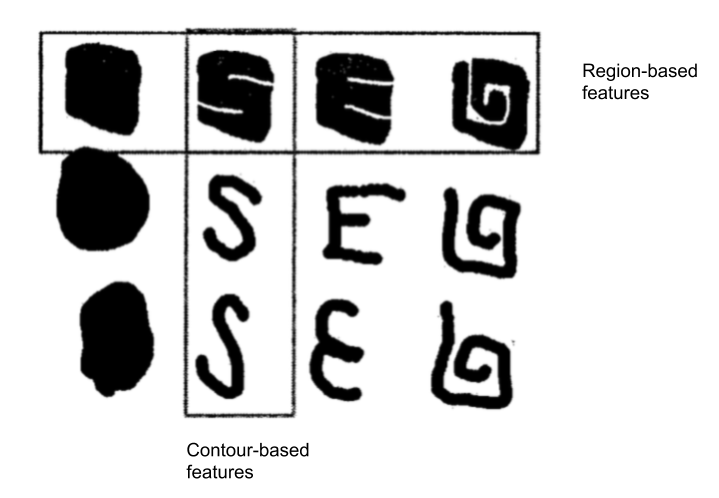
\includegraphics[height=5cm]{02_background/CBIR/shape_features}}
%\caption{\label{fig:shape_feat} \textbf{Shape Features}. The highlighted row shows images considered similar based on region shape feature, and the highlighted column shows contour-based similarity. Figure reprinted from \cite{bober_mpeg-7_2001}}.
%\end{figure}

Various methods for shape extraction have been developed, however, most of them have difficulties dealing with the projection of real world 3-D object onto a 2-D image and can also struggle with abnormalities created by lighting and shadows \cite{zhang2004review}.

\subsubsection{MPEG-7}
The MPEG-7 standards were developed to describe the contents of images, audio and video independently from their format. They provide various low-level feature descriptors of color, shape, texture, motion and others, that enable fast and efficient multimedia search \cite{noauthor_visual_nodate}.

Many of these descriptors are widely used in CBIR systems, such as the color layout, edge histogram or 3D shape descriptor.

\subsection{CNN Features}
Convolutional Neural Networks, also known as ConvNets or CNNs, are the state-of-the-art neural networks for most computer vision tasks, such as image classification or object detection. Various research has also shown that a ConvNet can produce very powerful image descriptors, which can be used for image retrieval \cite{razavian_cnn_2014-2}, \cite{NIPS2012_4824}.

Unlike regular feed-forward neural networks based on fully-connected layers of neurons, ConvNets are trained to learn relatively small filter kernels, that can extract relevant information from different areas of an image. Therefore, they reduce the amount of training parameters significantly and are able to train also on large images.

As shown in Figure \ref{fig:conv_feats}, in the early layers of the network, the filters learn to recognize simple visual features, such as horizontal edges or colors. These low-level feature are combined and create more complex structures as the network's layers get deeper. In the last layers of the network, the filters are trained to recognize high-level features, which can be used not only to classify the image, but also to describe it.

\begin{figure}[h]
\centering
\subcaptionbox{Low-Level Features}{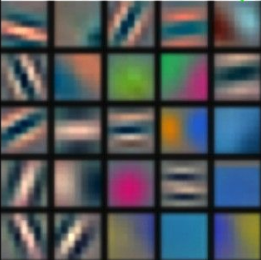
\includegraphics[height=4cm]{02_background/CBIR/feat_low}}\hspace{.3cm}
\subcaptionbox{Mid-Level Features}{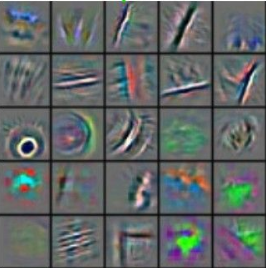
\includegraphics[height=4cm]{02_background/CBIR/feat_mid}}\hspace{.3cm}
\subcaptionbox{High-Level Features}{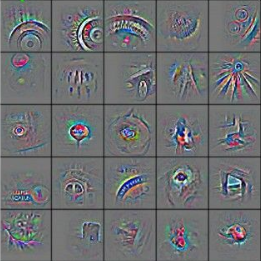
\includegraphics[height=4cm]{02_background/CBIR/feat_high}}
\caption{\label{fig:conv_feats} \textbf{Convolutional Feature Maps}. Each image displays a sample of feature maps (filters) from different layers of the networks. The early layer feature maps recognize simple patterns, while the last layers recognize more complex structures. Figure adapted from \cite{gandhi_build_2018}.}
\end{figure}


Krizhevsky et al. \cite{NIPS2012_4824} use a ConvNet, trained to classify more than 1 million images into 1000 classes, to extract 4028-dimensional image features from the last hidden layer of the network. They show, that these feature vectors can be used to find images with similar content and are invariant to the position of the objects in the image, lighting and colors. Their results are shown in Figure \ref{fig:conv_cbir}.


\pagebreak
\subsection{Distance Metrics}
To retrieve relevant images, distances between the extracted image features need to be evaluated based on a metric. The distance between two images should be small, if the images are similar and vice versa. 

The most commonly used metrics is the \textit{L1 norm}, also called \textit{Manhattan distance}, and \textit{L2 norm}, also known as \textit{Euclidean distance}.

Given two $n$-dimensional vectors vector $x = (x_1, x_2, ..., x_n)$ and $y = (y_1, y_2, ..., y_n)$, the L1 distance is computed by summing up the absolute values of the difference between the respective coordinates of the vectors:
\begin{equation}
L_1(x, y) = \sum_{i=1}^{n} |x_i - y_i|.
\end{equation} 

L2 distance is the squared root of sum of squared distances between respective vector coordinates:
\begin{equation}
L_2(x, y) = \sqrt{\sum_{i=1}^{n} (x_i - y_i)^2}.
\end{equation}

There are also other possible metrics like the \textit{Chebychev metric} or the \textit{Minkowski Metric}, however these metrics are not used for the purpose of this thesis. 


\pagebreak
% ==============================================================
\chapter{Analysis}
% ==============================================================
This chapter firstly introduces the fashion dataset used in this thesis, its requirements and comparison with other available datasets. As mentioned earlier, online fashion retail does not only provide a large amount of visual and textual data, but it is also a field where the search results should fit the individual style and taste of the user. Therefore, I chose this fashion data for the goal of this thesis - to evaluate how user-driven image synthesis can improve image retrieval.

Next, the chapter compares five existing image-to-image translation GANs that can be used for image synthesis, describes their architecture, usage and specific characteristics. I chose image-to-image translation models, since they are based on the concept of conditional generative adversarial networks, and therefore are able to be influenced by image input.

Finally, the chapter introduces several features for image retrieval, from low-level features to features produced by a convolutional neural network. These features can be used to retrieve similar images to both original and synthesized images.

Some of the existing implementations of generative adversarial networks specifically for fashion data are also mentioned at the end of the chapter.

% ==============================================================
% DATA
% ==============================================================
\section{Data} \label{sec:data}
As in most machine learning algorithms applied to visual tasks, the quantity and quality of training data is essential to produce high-quality results. It is also common, that data collection and data cleaning make up a significant part of a machine learning project.

In case of fashion images, there are several open-source datasets published online. However, after careful evaluation I have not found them sufficient for the purpose of this thesis. Therefore I have created an application to scrape online fashion stores and download images of fashion products and their description in a computer-readable format.

\pagebreak
% ==============================================================
\subsection{Requirements}
% ==============================================================

In order to generate high-quality outputs using GANs, the collected dataset should fulfill the following requirements:
\begin{enumerate}
\item The fashion products should be photographed on a white background. 
\item There should be a machine-readable description of each product, such as color, shape, category, etc. 
\item The images should be in a sufficient resolution.
\item There should be a sufficient amount of images of various items.

\end{enumerate}
I have defined these requirements based on my previous experience with generative algorithms. It is generally easier for the algorithm to focus on the important attributes of the images, if there are no distractions in terms of different model poses, backgrounds, etc. And since the main point of the project is to modify different attributes of the products, the images need to be labeled.

\subsection{Existing Fashion Datasets}
\paragraph{DeepFashion}
The DeepFashion dataset \cite{liu2016deepfashion} includes more than 200.000 images of clothing images, labeled with 1.000 attributes. However, this dataset does not fulfill the first requirement of the dataset - its clothing items are photographed on people in various poses and backgrounds, as shown in Figure \ref{fig:deepfashion}. This type of variation might be too complex for the algorithms and can lead to unsatisfactory results.

\begin{figure}[h]
\centering
{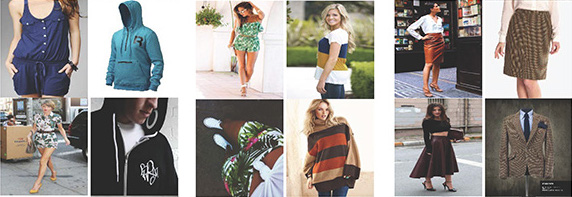
\includegraphics[width=\linewidth]{03_analysis/data/deepfashion}}
\caption{\label{fig:deepfashion} \textbf{DeepFashion Dataset}. Figure reprinted from \cite{liu2016deepfashion}.}
\end{figure}

\paragraph{Fotolia}
Another available dataset, that has been provided by my supervisors, is the Fotolia  dataset \cite{noauthor_fotolia_nodate}. It contains more than 20 million tagged images with large variety of objects, among which are also fashion products, and can be explored on the PicsBuffet website \cite{mackowiak_picsbuffet_nodate}.

To test the dataset, I have chosen all images with keywords ,,dress'' and ,,isolated'' and compared them to a template image, based on the distance between their 64-dimensional feature vectors (calculated via Akiwi API \cite{sonnenberg_akiwi_nodate}). Figure \ref{fig:fotolia} shows the results of this search. 

Additionally to an undesired low resolution of the returned images - around 100 x 160 pixels - the results also have too much variety, such as different model poses, different zoom levels and backgrounds. The description of the images did not include many useful attributes, with most pictures being labeled with words such as: ,,beauty'', ,,young'', ,,person'', and lacking information about colors, shapes and pattern.

\begin{figure}[h]
\centering
\subcaptionbox{Template Image}{\fbox{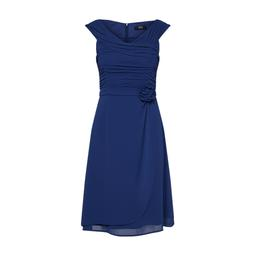
\includegraphics[height=3.5cm]{03_analysis/data/dress_template}}}\hspace{1cm}
\subcaptionbox{Fotolia Images}{\fbox{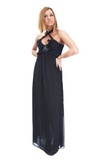
\includegraphics[height=3.5cm]{03_analysis/data/fotolia_ex1}}
\fbox{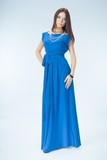
\includegraphics[height=3.5cm]{03_analysis/data/fotolia_ex2}}
\fbox{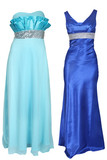
\includegraphics[height=3.5cm]{03_analysis/data/fotolia_ex3}}}
\caption{\label{fig:fotolia} \textbf{Fotolia images.} The retrieved Fotolia images (b) with keywords ,,dress'' and ,,isolated'' with smallest feature vector distance from the template image (a).}
\end{figure}


% ==============================================================
\subsection{Scraped Dataset}
% ==============================================================
Based on the evaluation of existing fashion datasets, I have identified a need for creating a new dataset specifically for the requirements of the application. I evaluated several online fashion retailers that provide downloadable product images and easily parsable descriptions. 

I chose three websites, based on the structure and amount of information they provide: \href{https://www.zalando.de/damen-home/}{zalando.de}, \href{https://www.aboutyou.de/}{aboutyou.de} and \href{https://www.fashionid.de/damen/}{fashionid.de}. Each of them offer several thousand fashion products for women and men, with a photograph of the item on a white background and some basic description such as color, pattern, shape, length etc. For simplicity, I have limited the dataset to women's clothes, excluding products like accessories and shoes.

The \textit{Fashion Scraper} is a python project, that scrapes images and data from all the mentioned websites and saves them locally for further processing, such as image processing, data cleaning, and description translating. This project was part of my Independent Coursework and the source code of the project can be found on \href{https://github.com/sonynka/fashion_scraper}{github.com/sonynka/fashion\_scraper}.

\begin{figure}[h]
\centering
{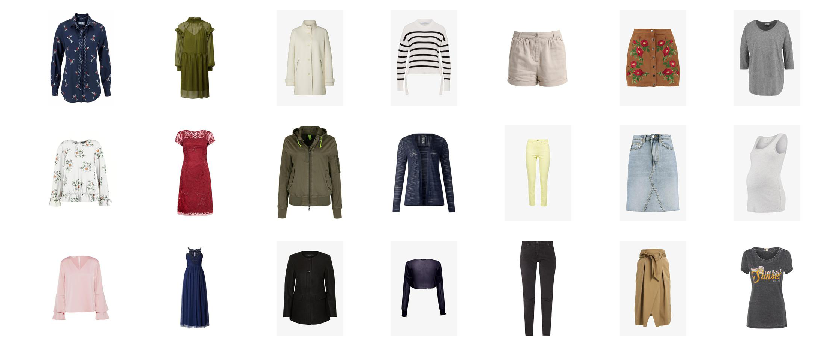
\includegraphics[width=\linewidth]{03_analysis/data/img_grid2}}
\caption{\label{fig:dataset} \textbf{Examples of images in the final dataset.} Each column contains images from different category as follows: blouses, dresses, jackets, knitwear, pants, skirts, tops.}
\end{figure}

The scraped dataset consists of 92.200 images of size $256\times256$ pixels in JPEG format. The images are split into folders by categories and the whole dataset is described in a CSV file, which includes information such as ID of the product,  path to the image file, URLs to image files hosted on the website, product brand etc.
%\begin{itemize}
%\item \textbf{id}: ID of the product as defined by the website (SKU)
%\item \textbf{img\_path}: relative local file path to the saved product image
%\item \textbf{img\_url}: URL to the product image file hosted on the seller website
%\item \textbf{model\_img\_urls}: URLs to the images of the product worn by models
%\item \textbf{product\_url}: if given, the URL to the product listing on the website
%\item \textbf{brand}: product brand as displayed on the website
%\item \textbf{name}: product name as displayed on the website
%\item \textbf{attributes}: list of product attributes listed on the website in German, such as shape, length, material, size etc.
%\end{itemize}

In addition to the website data, there are columns that contain processed and translated data. Below is the list of the column names and their respective possible values.
\begin{itemize}
\item \textbf{category}: blouses, dresses, jackets, knitwear, pants, skirts, tops
\item \textbf{color}: beige, black, blue, gray, green, pink, red, white, yellow
\item \textbf{length}: 3-4, knee, long, normal, short or no value
\item \textbf{sleeve\_length}: half, long, short, sleeveless or no value
\item \textbf{fit}: loose, normal, tight or no value
\item \textbf{pattern}: floral, lace, polkadots, print, stripes, unicolors or no value
\item \textbf{neckline}: back, deep, lines, round, v, wide or no value
\end{itemize}

\pagebreak
\paragraph{Model Images}
For each scraped product, I also downloaded images of the product worn by models. The model images are of size $256\times256$ pixels in JPEG format and the file names correspond to the file names of the product images. Each product has variable amount of corresponding model images, varying in model poses, zoom level and detail level of the photo (see Figure \ref{fig:models}).

\begin{figure}[h]
\centering
{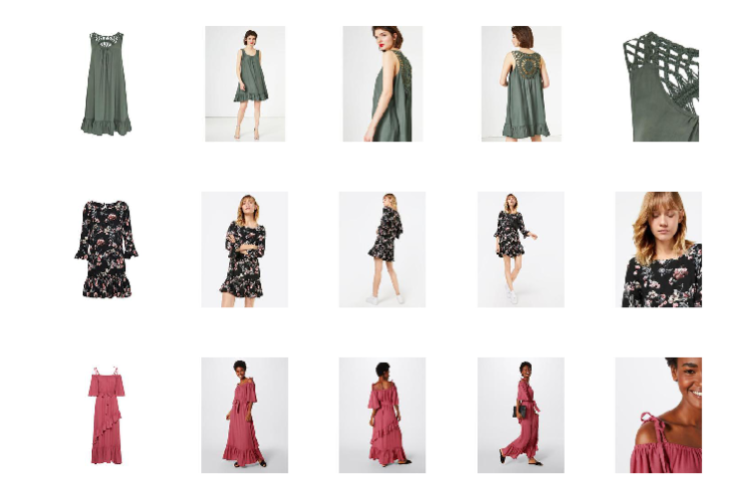
\includegraphics[width=\linewidth]{03_analysis/data/model_images}}
\caption{\label{fig:models} \textbf{Examples of model images in the dataset.} First column shows the product images and the other columns show images of models wearing the given product in various poses and level of detail.}
\end{figure}

\pagebreak
% ==============================================================
\section{Image-To-Image Translation}
% ==============================================================
Image-To-Image Translation using GANs has been widely researched in the past few years, with creative approaches and models published regularly. For the purpose of this thesis, I have reviewed and tested some of these projects, to evaluate what results can be achieved on the fashion dataset and which GAN is best suited for what task.

Table \ref{tab:gan_comp} shows the comparison of 5 evaluated networks: pix2pix \cite{isola_image--image_2016}, CycleGAN \cite{zhu_unpaired_2017}, StarGAN \cite{choi_stargan_2017}, MUNIT \cite{huang_multimodal_2018} and FaderNetworks \cite{lample_fader_2017}, for which I compared the following attributes:
\begin{itemize}
\item \textbf{Supervised}: Does the network require a dataset consisting of paired images, such as the same skirt in a short and long version.
\item \textbf{Multi-Domain}: Is the network able to train one model for different domains translations, or does each domain pair require an individually trained generator.
\item \textbf{Multi-Modal}: Is the network able to generate diverse outputs from the same input.
\item \textbf{Latent representations}: Does the network train in pixel-space or uses latent representations, such as separate content and style representations.
\end{itemize}

The following sections describe the characteristics of the evaluated networks, their applications, training process and architecture.

\begin{table}[h]
\centering
\begin{tabular}{l*{5}{c}}
Characteristics & pix2pix &	CycleGAN & StarGAN	& MUNIT	& FaderNets \\
\hline
Supervised				& \checkmark 	& $\times$ & $\times$ 	& $\times$ 	& $\times$ \\
Multi-Domain  			& $\times$  	 	& $\times$ & \checkmark 	& $\times$ 	& $\times$ \\
Multi-Modal				& $\times$ 		& $\times$ & $\times$ 	& \checkmark & $\times$ \\
Latent Space 			& $\times$ 		& $\times$ & $\times$ 	& \checkmark & \checkmark \\
\end{tabular}
\caption{\label{tab:gan_comp}\textbf{Comparison of existing GAN models based on their characteristics.} %Supervised training means that the dataset consists of image pairs, e.g: a dress and a person wearing the dress. Multi-Domain networks are able to train one model to change multiple attributes. Multi-Modal networks are able to generate more than one possible output. Networks with latent representations try to model the training data in a latent space, as opposed to pixel space.
}
\end{table}

\pagebreak
\subsection{Pix2Pix} \label{sec:pix2pix}
The so-called Pi2Pix networks were first introduced by Isola et al. \cite{isola_image--image_2016} as a framework for image-to-image translations. Some of the applications of Pix2Pix include mapping day photographs to night, translating sketches of shoes to realistic shoe images or colorizing black-and-white photos (Figure \ref{fig:pix2pix_example}).

\begin{figure}[h]
\centering
{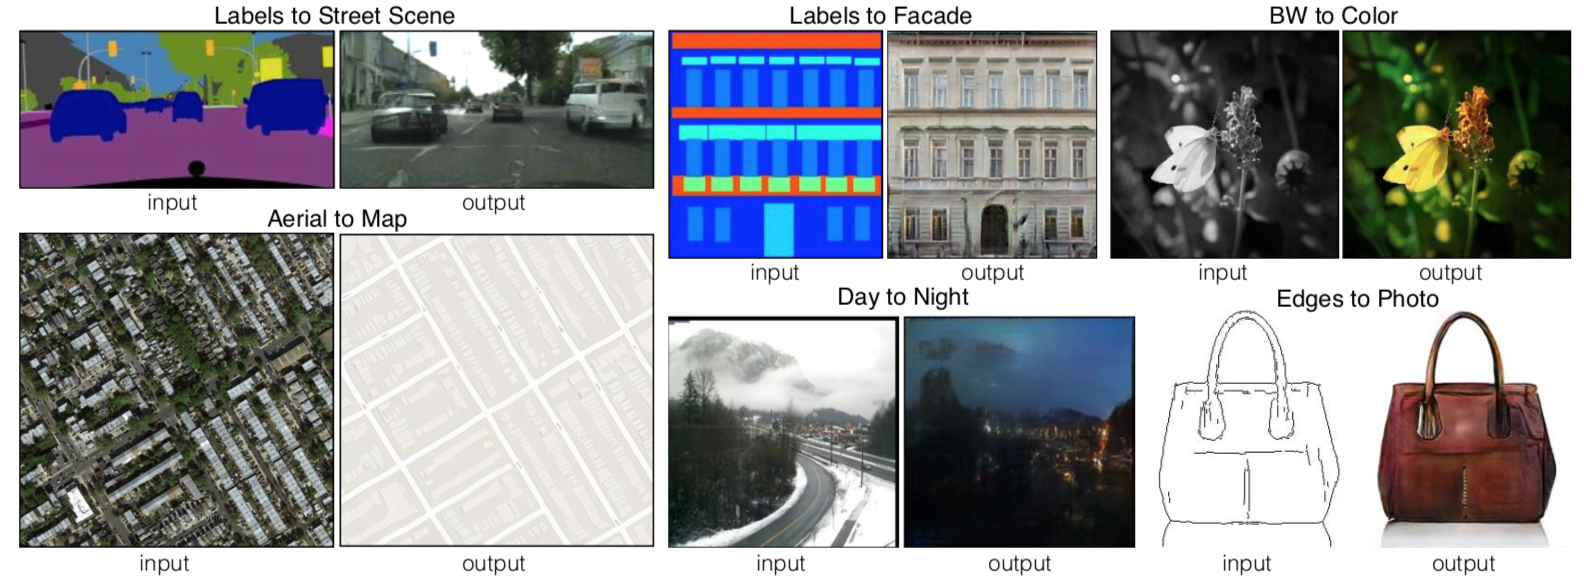
\includegraphics[width=\linewidth]{03_analysis/gans/pix2pix_example}}
\caption{\label{fig:pix2pix_example} \textbf{Pix2Pix: Examples of translation between various domains.} Use cases of the pix2pix framework include translating day images to night or colorizing grayscale images. Figure reprinted from \cite{hesse_image--image_2017}.}
\end{figure}

Pix2Pix uses the concept of conditional GANs \cite{mirza_conditional_2014} (described in Section \ref{sec:cond_gan}) to influence the network's output by providing a condition. In case of Pix2Pix, the condition is an image that should be translated to another domain. To translate images from an input domain to a target domain, the model requires a dataset of paired images $(x_{input}, x_{target})$, such as a grayscale image and a corresponding color image. 


\begin{figure}[h]
\centering
{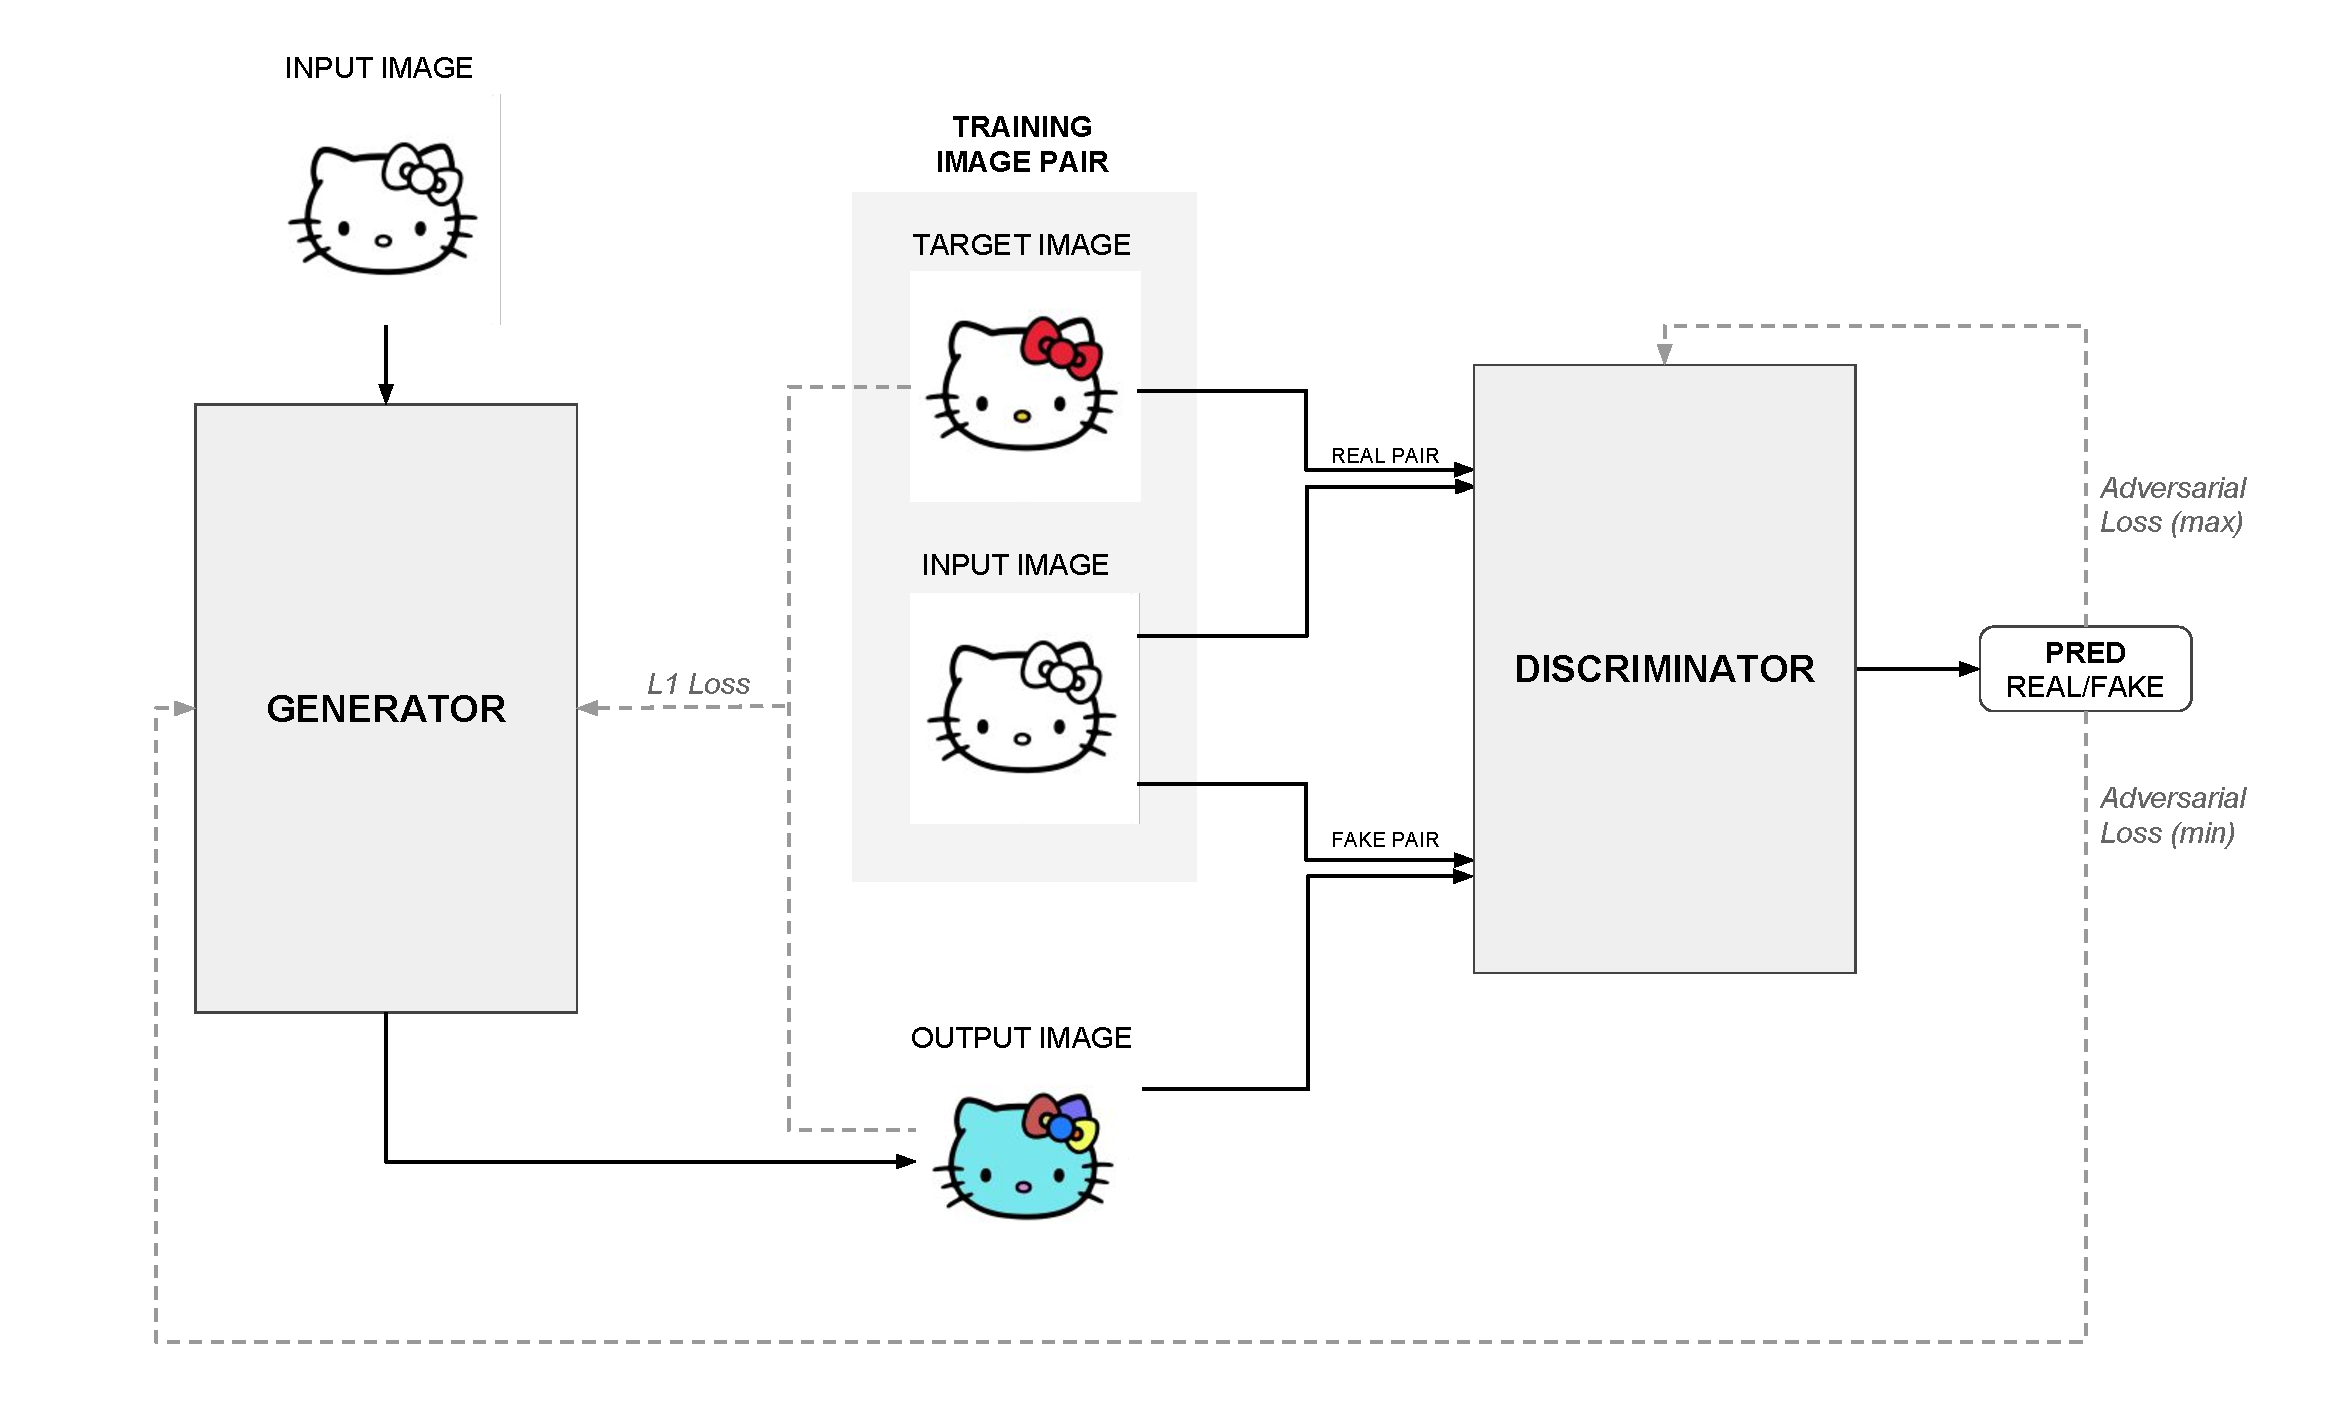
\includegraphics[width=\linewidth]{03_analysis/gans/pix2pix}}
\caption{\label{fig:pix2pix} \textbf{Pix2Pix Training Process.} Dataset consists of paired input and target images. Generator takes input image as condition to output a generated image. Discriminator tries to predict, given the input image, if the target image comes from dataset or from generator. This output is then used to further optimize both networks. Figure adapted from \cite{hesse_image--image_2017}.}
\end{figure}

As shown in Figure \ref{fig:pix2pix}, the generator takes the input image $x_{input}$ and tries to map it to the target domain $\hat{x}_{target}$, such as: $G: (x_{input}) \rightarrow \hat{x}_{target}$. The discriminator, also conditioned on the input image $x_{input}$, tries to predict if the target image comes from the data distribution or if it was generated. The discriminator tries to improve these classifications, while the generator tries to prevent correct classification.


\paragraph{Training Objective}
The adversarial objective, which $G$ is trained to minimize and $D$ is trained to maximize, can be expressed as following:
\begin{equation}
\underset{G}{\mathrm{min}} \ \underset{D}{\mathrm{max}} \ \mathcal{L}_{adv}(D,G) = \mathbb{E}_{x_{in},x_{trg}}[\log D(x_{in},x_{trg})] + \mathbb{E}_{x_{in}}[\log 1 - D(x_{in}, G(x_{in}))]
\label{eq:pix2pix_minimax_cond}
\end{equation}

\pagebreak
Based on the results of previous conditional GAN approaches \cite{pathak_context_2016}, Isola et. al \cite{isola_image--image_2016} have also shown, that enforcing the generated output to be closer to the ground truth target by adding a second objective reduces artifacts in the results. They therefore suggest to use the L1 distance as reconstruction loss function for the generator to optimize.
\begin{equation}
\mathcal{L}_{rec}(G) = \mathbb{E}_{x_{in},x_{trg}}[||x_{trg}-G(x_{in})||_{1}]
\label{eq:pix2pix_loss_rec}
\end{equation}

The final objective of the generator is:
\begin{equation}
\mathcal{L} = arg \ \underset{G}{\mathrm{min}} \ \underset{D}{\mathrm{max}} \ \mathcal{L}_{adv}(D,G) + \lambda \mathcal{L}_{rec}(G)
\end{equation}
where $\lambda$ controls the relative importance of the two loss functions.


\paragraph{Generator}
In image translation tasks, it is usual, and even desirable, that the input and target image domains share a common underlying structure. Modeling the generator with a simple encoder-decoder architecture, where all data must pass through a so-called ,,bottleneck'' layer, can therefore result in an undesirable loss of the low-level details that the two domains share. 

The authors therefore suggest to base the generator on a U-Net architecture. U-Net contains so-called skip connections, which pass the output directly from the encoder to the decoder, skipping the bottleneck. The generator is therefore able to include low-level features from the input in the output.

\begin{figure}[h]
\centering
{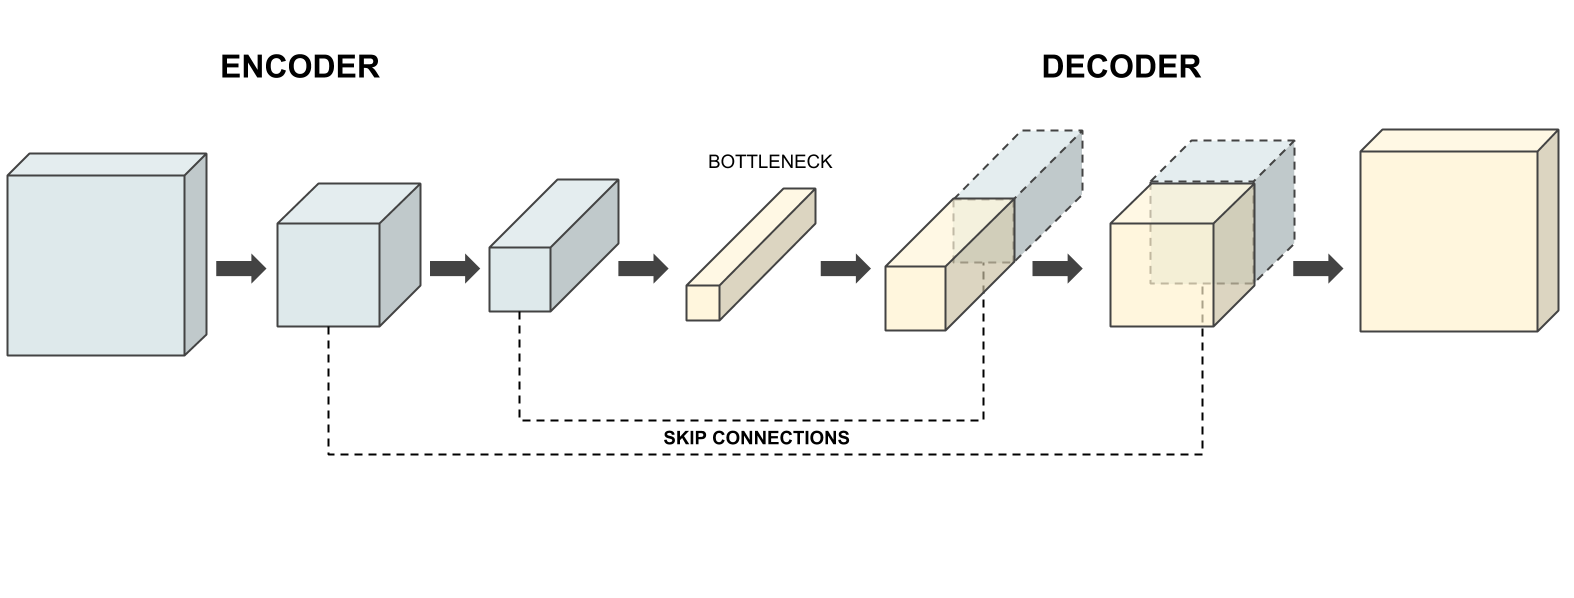
\includegraphics[width=\linewidth]{03_analysis/gans/u-net}}
\caption{\label{fig:u-net} \textbf{U-Net Generator.} Skip connections are added between each encoder layer $i$ and decoder layer $n - i$, where $n$ is the total number of layers, so that information can bypass the bottleneck.}
\end{figure}

\paragraph{Discriminator} \label{sec:patchgan}
The authors of Pix2Pix \cite{isola_image--image_2016} argue, that while the use of L1 or L2 loss for image generation usually produces blurry outputs, they are sufficient to capture low-level frequencies, for example the colorfulness of the image. Therefore, when combining adversarial loss with an L1 loss, the discriminator only needs to focus on high-level frequencies. 

They introduce the \textit{PatchGAN} architecture - a discriminator, which evaluates the high-frequency structure of the input image in patches. The PatchGAN discriminator can be described as a convolution running over the input image, classifying each patch as real or fake. The overall classification of an image is then calculated as the average of the decision for each patch. This allows the discriminator to scale efficiently to larger images and, as the authors have shown, forces sharp and colorful outputs.


%\paragraph{Usage}
%The distinct feature of Pix2Pix among the evaluated networks is that the training process is supervised. In case of the fashion dataset, there are not a lot of examples of paired images from two domains, e.g: images of the same products with long sleeves and with short sleeves.

\pagebreak
\subsection{CycleGAN}
CycleGANs \cite{zhu_unpaired_2017}, unlike Pix2Pix, do not require a paired image set for the image domains to be translated. The unsupervised setting is preferred in most translation tasks, as obtaining image pairs of two domains can be difficult or even impossible - for example translating female faces to male, or Monet artworks to realistic photographs. The assumption hereby is that both image domains share certain underlying visual similarities.

\begin{figure}[h]
\centering
{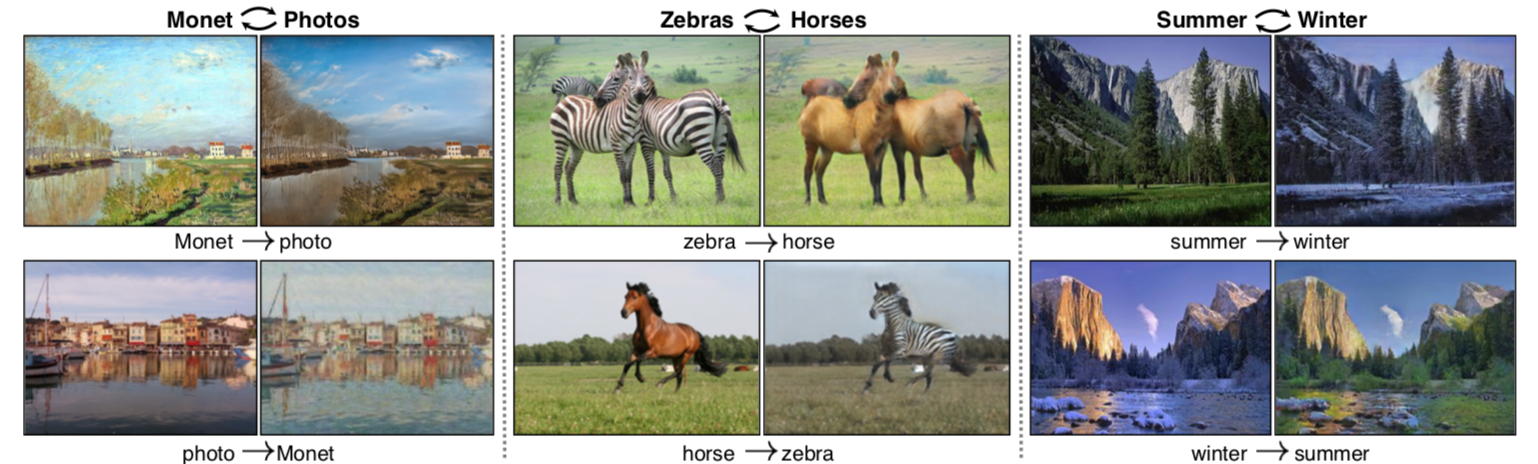
\includegraphics[width=\linewidth]{03_analysis/gans/cyclegan_example}}
\caption{\label{fig:cyclegan_examples} \textbf{CycleGAN: Examples of translations between various domains.} Examples of bi-directional mappings between photography and Monet artworks, zebras and horses and summer and winter images. Figure reprinted from \cite{zhu_unpaired_2017}.}
\end{figure}

The model consists of two generators, $G_{X}$ and $G_{Y}$, which learn mapping from image domain $X$ to image domain $Y$, $G_{Y}: X \rightarrow Y$, and vice versa, $G_{X}: Y \rightarrow X$. Each of the image domains has its own discriminator, $D_{X}$ and $D_{Y}$, that check if the given image comes from the real distribution of the domain or is translated from the opposite domain.

\paragraph{Adversarial Loss}
The adversarial loss is applied to both pairs of networks, $(D_{X}, G_{X})$ and $(D_{Y}, G_{Y})$.
\begin{equation}
\mathcal{L}_{adv}(D_{X},G_{X}) = \mathbb{E}_{x}[\log D_{X}(x)] + \mathbb{E}_{y}[\log 1 - D_{X}(G_{X}(y))]
\label{eq:cyclegan_adv}
\end{equation}

\paragraph{Cycle Consistency Loss}
Additionally to the adversarial loss, CycleGAN also implements a so-called \emph{Cycle Consistency Loss}, which enforces that an image encoded from one domain to another, can also be reconstructed back to the original domain. The authors argue, that reducing the amount of possible mapping functions can help avoid the network to learn mappings that contradict each other \cite{zhu_unpaired_2017}.

\pagebreak
The \textit{forward cycle consistency} defines that an image $x$ from domain $X$ and its encoded-decoded version should be approximately the same: $G_{X}(G_{Y}(x)) \approx x$. The \textit{backward cycle consistency} defines the same for an image from domain $Y$.
\begin{equation}
\mathcal{L}_{cyc}(G_{X},G_{Y}) = \mathbb{E}_{x}[||G_{X}(G_{Y}(x)) - x||_{1}] + \mathbb{E}_{y}[||G_{Y}(G_{X}(y)) - y||_{1}]
\label{eq:cyclegan_cycle}
\end{equation}


\begin{figure}[t]
\centering
\subcaptionbox{CycleGAN Model}
{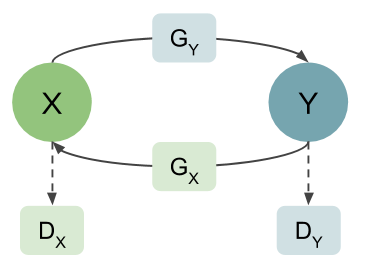
\includegraphics[height=4cm]{03_analysis/gans/cyclegan1}}\hspace{1cm}
\subcaptionbox{Cycle Consistency Loss}
{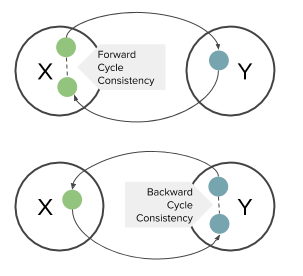
\includegraphics[height=4cm]{03_analysis/gans/cyclegan2}}
\caption{\label{fig:cyclegan} \textbf{CycleGAN} (a) The model consists of two mappings, $G_{X}$ and $G_{Y}$ and corresponding discriminators $D_{X}$ and $D_{Y}$. (b) Cycle Consistency Loss measures the L1 distance between a real sample from one image domain and its encoded-decoded version. Figure adapted from \cite{zhu_unpaired_2017}.}
\end{figure}


\paragraph{Training Objective}
Both generators train to minimize and both discriminators train to maximize the final objective, which regulates the relative weight of the adversarial loss against the cycle consistency loss with the hyperparameter $\lambda$.
\begin{equation}
\begin{split}
G^{*}_{X}, G^{*}_{Y} = arg \ \underset{G_{X}, G_{Y}}{\mathrm{min}} \ \underset{D_{X}, D_{Y}}{\mathrm{max}} \ \mathcal{L}_{adv}(D_{X},G_{Y}) \ +  \mathcal{L}_{adv}(D_{Y}, G_{X}) \\ + \ \lambda \mathcal{L}_{cyc}(G_{X}, G_{Y})
\end{split}
\end{equation}

\paragraph{Architecture}
CycleGAN models are roughly based on Deep Convolutional GANs \cite{radford_unsupervised_2015}, using the PatchGAN architecture \cite{isola_image--image_2016} for the discriminator.


\pagebreak
% =======================================================================
\subsection{StarGAN}
% =======================================================================

One of the disadvantages of Pix2Pix and CycleGAN is the missing possibility of multi-domain translation. If there are more than 2 domains to translate between, one must train a new model for each domain pair. This can be time and computationally intensive.

StarGAN \cite{choi_stargan_2017} is unique among the tested models, as it is able to train one single generator that maps input to multiple domains, as shown in Figure \ref{fig:stargan_topo}. Using the conditional GAN model \cite{mirza_conditional_2014}, the generator is conditioned on a randomly chosen target domain each iteration, so that it can learn mapping for all given domains. %StarGAN does not require paired image examples, however, the images need to be labeled in order to be separated into different domains.

\begin{figure}[h]
\centering
\subcaptionbox{Cross-Domain Models}
{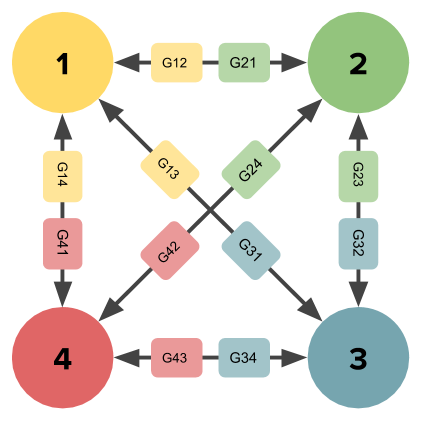
\includegraphics[height=4cm]{03_analysis/gans/StarGAN_graph}}\hspace{1cm}
\subcaptionbox{StarGAN Model}
{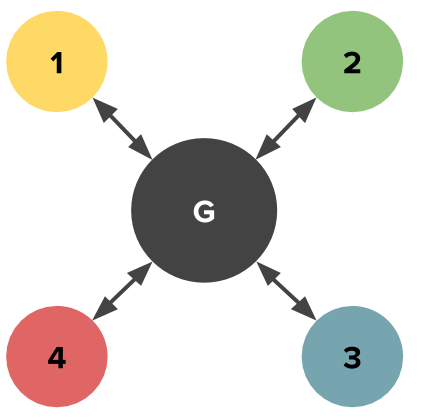
\includegraphics[height=4cm]{03_analysis/gans/StarGAN_graph2}}
\caption{\label{fig:stargan_topo} \textbf{Comparison of cross-domain models and StarGAN model.} While cross-domain models need one generator per each domain pair, StarGAN only trains one generator for multiple domains. Figure adapted from \cite{choi_stargan_2017}.}
\end{figure}

The overall training objective of StarGAN consists of three loss functions:
\begin{itemize}
\item \textit{Domain Classification Loss}, which forces the discriminator to also output the domain class of the input image,
\item \textit{Adversarial Loss}, which is maximized by the discriminator and minimized by the generator,
\item \textit{Cycle Consistency Loss}, which measures the distance between an original image and its version encoded-decoded by the generator.
\end{itemize}

\begin{figure}[h]
\centering
{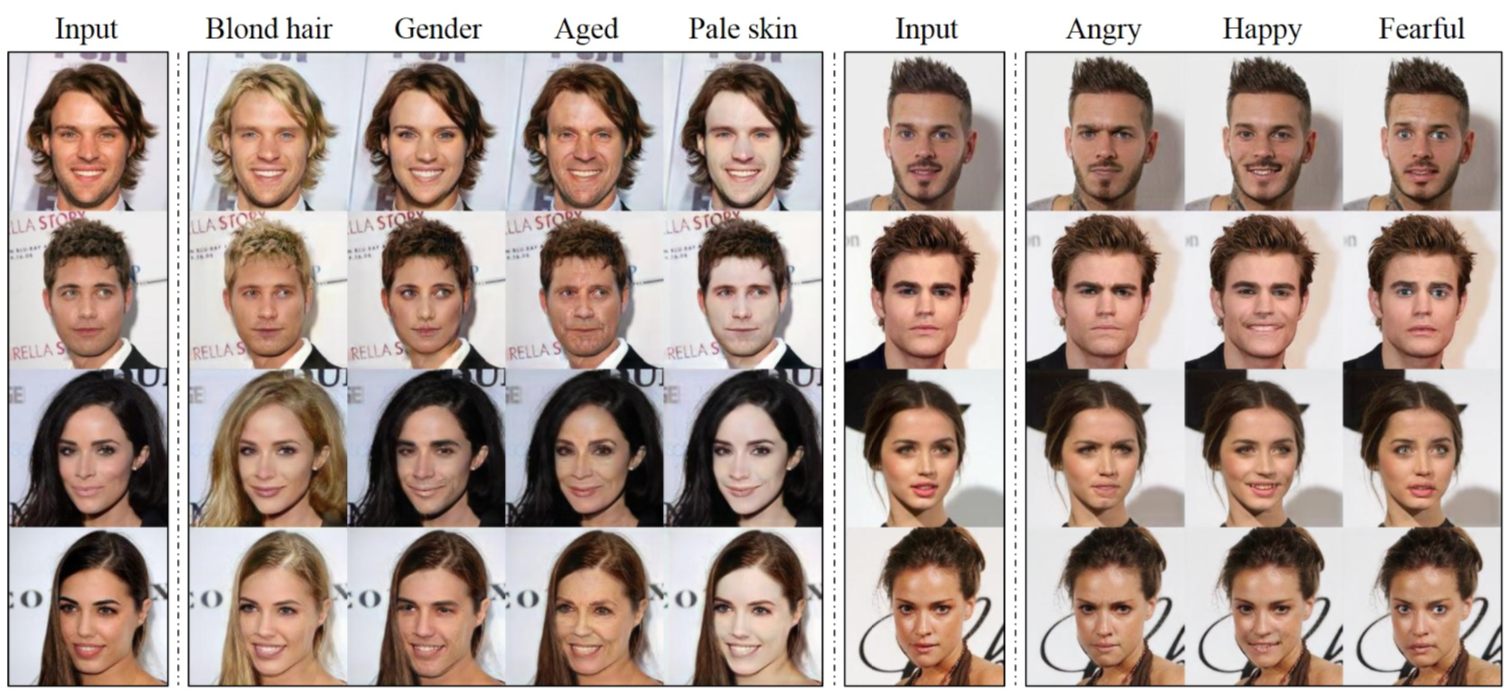
\includegraphics[width=.8\linewidth]{03_analysis/gans/stargan_example}}
\caption{\label{fig:stargan_examples} \textbf{StarGAN: Examples of translations based on various attributes.} First and sixth columns show the input image, the rest columns show modified versions based on the given attribute. Figure reprinted from \cite{choi_stargan_2017}.}
\end{figure}

\paragraph{Domain Classification Loss} 
Instead of feeding the target domain class $c$ to the discriminator, as in common conditional networks, StarGAN trains the discriminator to classify it. It uses an auxiliary classifier GAN, AC-GAN \cite{odena_conditional_2016}, which forces the discriminator to output both the probability distribution over the sources of the input, and the probability of the target domain labels, $D: x \rightarrow {D_{src}(x), D_{cls}(x)}$. This improves the network's stability and performance, as it forces the discriminator to perform and additional task.

This modification to the discriminator introduces the \textit{Domain Classification Loss} with two objectives, ${L}^{r}_{cls}$ and ${L}^{f}_{cls}$, optimizing $D$ and $G$ respectively. Given training data with an image $x$ and its original domain $c_{in}$, $D$ learns to classify the domain label correctly by minimizing the following objective:
\begin{equation}
\mathcal{L}^{r}_{cls} = \mathbb{E}_{x,c_{in}}[-\log D_{cls}(c_{in}|x)].
\label{eq:stargan_clsr}
\end{equation}

The generator objective is to generate images, that fool the auxiliary classifier and are classified as the target domain $c_{trg}$:
\begin{equation}
\mathcal{L}^{f}_{cls} = \mathbb{E}_{x,c_{trg}}[-\log D_{cls}(c_{trg}|G(x, c_{trg}))].
\label{eq:stargan_clsf}
\end{equation}

\begin{figure}[h]
\centering
{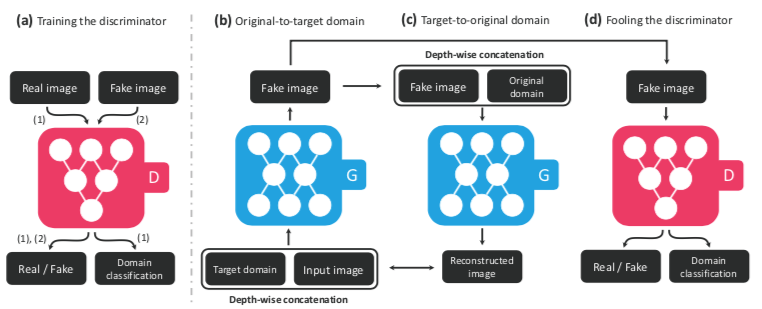
\includegraphics[width=\linewidth]{03_analysis/gans/stargan}}
\caption{\label{fig:stargan_training} \textbf{StarGAN Training Process.} The discriminator classifies the input as real or fake and outputs it's domain class prediction. The generator encodes the image with a target domain, and then decodes the output with the original domain, to calculate the cycle consistency distance. Figure reprinted from \cite{choi_stargan_2017}.}
\end{figure}

\paragraph{Adversarial Loss}
Given an image $x$ and a target domain label $c_{trg}$, generator $G$ tries to minimize the adversarial loss objective, to generate real-looking images conditioned on the target domain, while the discriminator classifying the source of the image, $D_{src}$, tries to maximize it.
\begin{equation}
\mathcal{L}_{adv} = \mathbb{E}_{x}[\log D_{src}(x)] + \mathbb{E}_{x, c_{trg}}[\log 1 - D_{src}(G(x, c_{trg}))]
\label{eq:stargan_adv}
\end{equation}

\paragraph{Cycle Consistency Loss}
Cycle Consistency Loss \cite{zhu_unpaired_2017} is used to generate images that preserve the underlying content of the original image, and only change the domain-related attributes:
\begin{equation}
\mathcal{L}_{cyc} = \mathbb{E}_{x,c_{in},c_{trg}}[||x - G(G(x,c_{trg}), c_{in})||_{1}].
\label{eq:stargan_cyc}
\end{equation}

\paragraph{Training Objective}
The full training objective for $D$ and $G$ respectively is:
\begin{equation}
\mathcal{L}_{D} = -\mathcal{L}_{adv} + \lambda_{cls} \mathcal{L}^{r}_{cls},
\label{eq:stargan_D}
\end{equation}
\begin{equation}
\mathcal{L}_{G} = \mathcal{L}_{adv} + \lambda_{cls} \mathcal{L}^{f}_{cls} + \lambda_{cyc} \mathcal{L}_{cyc},
\label{eq:stargan_G}
\end{equation}

where $\lambda_{cls}$ and $\lambda_{cyc}$ control the relative importance of the two loss functions against the adversarial loss.

The model architecture is based on CycleGAN.


\pagebreak
% ==============================================================
\subsection{MUNIT}
% ==============================================================

All of the introduced models approach the image translation problem as one-to-one mapping. However, many of the image domain translation tasks are in fact multi-modal, meaning one single input can have multiple different outputs. The MUNIT network \cite{huang_multimodal_2018} introduces an unsupervised multi-modal method, which is able to capture the diversity of the output, as shown in Figure \ref{fig:munit_example}.

Instead of using translation in pixel space, the model tries to model the translation in a latent space. Based on the \textit{partially shared latent space assumption}, a content latent code $c \in \mathcal{C}$ and a style latent code $s_{i} \in \mathcal{S}_{i}$ are separated, assuming that the two image domains share a common content space but each has an individual style space. 

\begin{figure}[h]
\centering
{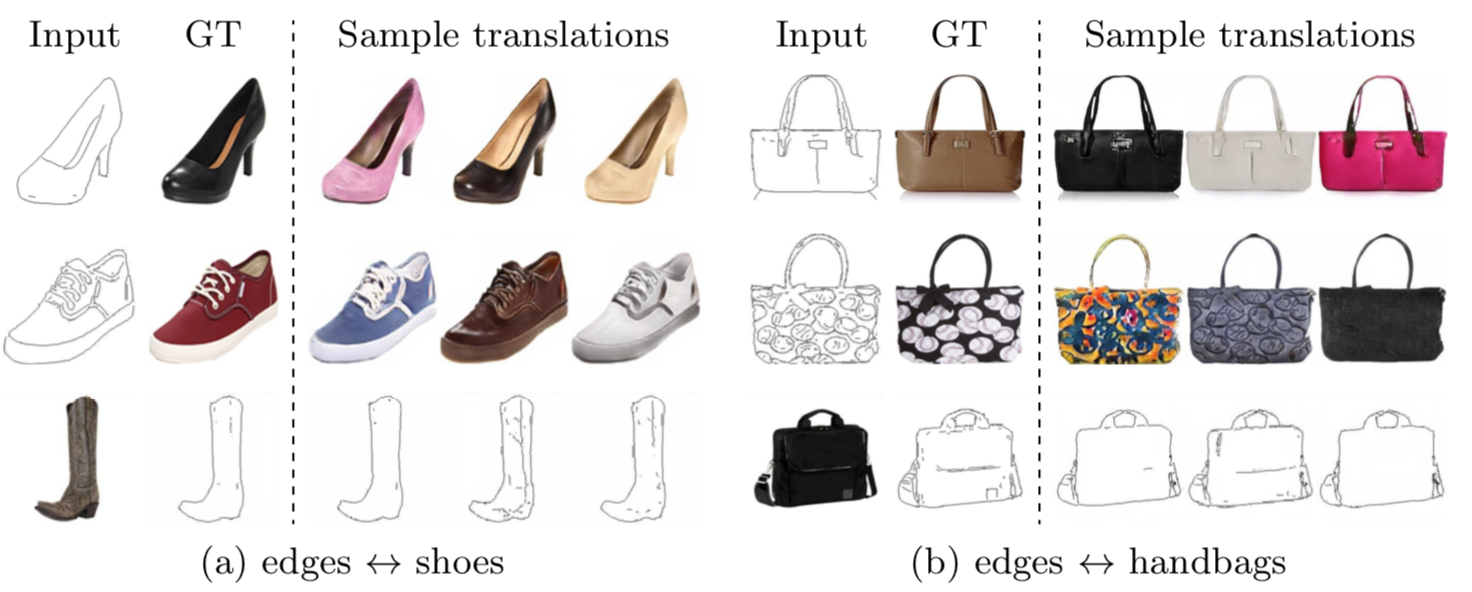
\includegraphics[width=\linewidth]{03_analysis/gans/munit_example}}
\caption{\label{fig:munit_example} \textbf{MUNIT: Examples of multi-modal translations.} For both translations, the input and ground-truth image are shown in the first two columns and the rest shows various generated samples. Figure reprinted from \cite{huang_multimodal_2018}.}
\end{figure}


For each domain, there is an auto-encoder, which consists of a generator $G$ and two encoders: content encoder $E^c$, and style encoder $E^s$. Given an image $x \in X$, it is encoded into a content and style code, $E^c_x(x)$ and $E^s_x(x)$. To translate the image $x \in X$ to domain $Y$, its content code $c_{x}$ is extracted using the content encoder $E^c_x$, and it is combined with a random style code $s_{y}$, $G_y(c_x, s_y)$. 

While the style code is assumed to have a global and simple effect and is therefore sufficiently represented by a low-dimensional vector, the content is assumed to be a high-dimensional vector describing the complex spatial structure of the data. Figure \ref{fig:munit_enc} shows the encoding of an image from domain $X$ to style and content code and the decoding back to the image domain.

\begin{figure}[h]
\centering
{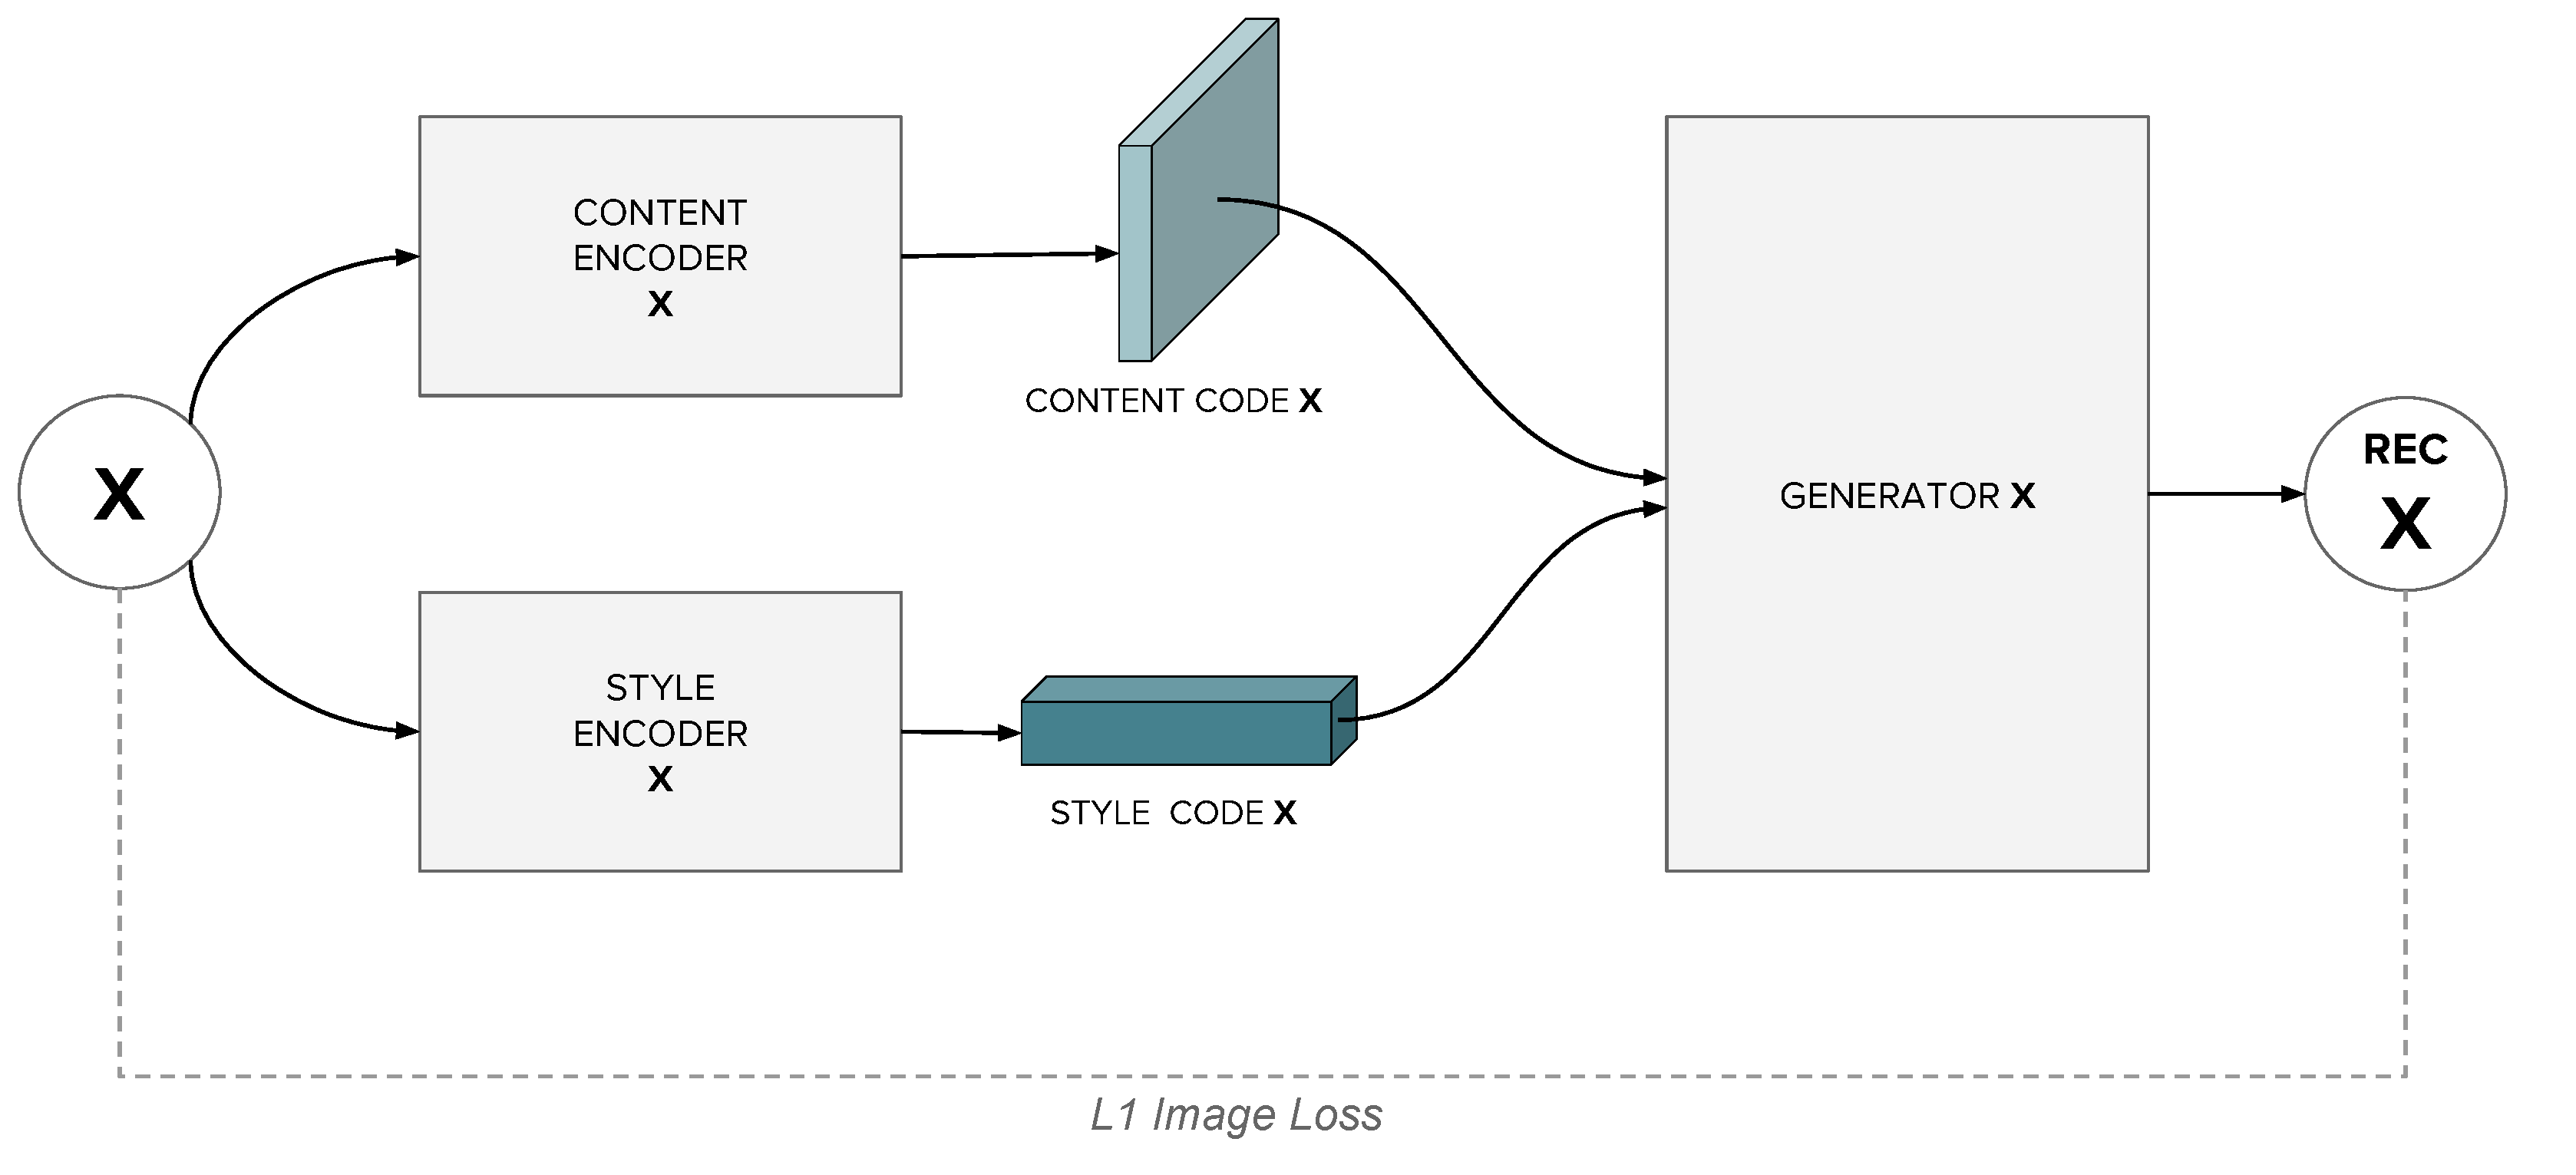
\includegraphics[width=\linewidth]{03_analysis/gans/munit_enc}}
\caption{\label{fig:munit_enc} \textbf{MUNIT within-domain reconstruction.}  An image from domain X is decomposed into content and style code via respective encoders. The decoder is a generator that combines the two latent encodings and translates them back to the original domain. A reconstruction loss is calculated between the original and the reconstructed image to optimize the auto-encoders. Figure adapted from \cite{huang_multimodal_2018}.}
\end{figure}

\paragraph{Reconstruction Loss}
The reconstruction loss is similar to the cycle consistency loss \cite{zhu_unpaired_2017}, enforcing the reconstruction between an image and its latent representation in both directions. 

The \textit{image reconstruction loss} encourages the reconstruction of an image after encoding to latent space and decoding back to image space.
\begin{equation}
\mathcal{L}^{x}_{rec} = \mathbb{E}_{x}[||x - G_{x}(E^{c}_{x}(x), E^{s}_{x}(x))||_{1}]
\end{equation}

The \textit{latent reconstruction loss} consists of a style loss and a content loss, which should be reconstructed after being encoded to image space and decoded back. The content loss enforces the preservation of semantic information of the translated image, while the style loss encourages diversity in the translated outputs.
\begin{equation}
\mathcal{L}^{c_{x}}_{rec} = \mathbb{E}_{c_{x}, s_{y}}[||c_{x} - E^{c}_{y}(G_{y}(c_{x},s_{y}))||_{1}]
\end{equation}
\begin{equation}
\mathcal{L}^{s_{y}}_{rec} = \mathbb{E}_{c_{x}, s_{y}}[||s_{y} - E^{s}_{y}(G_{y}(c_{x},s_{y}))||_{1}]
\end{equation}

The same losses are also applied to image domain $Y$.

\begin{figure}[h]
\centering
{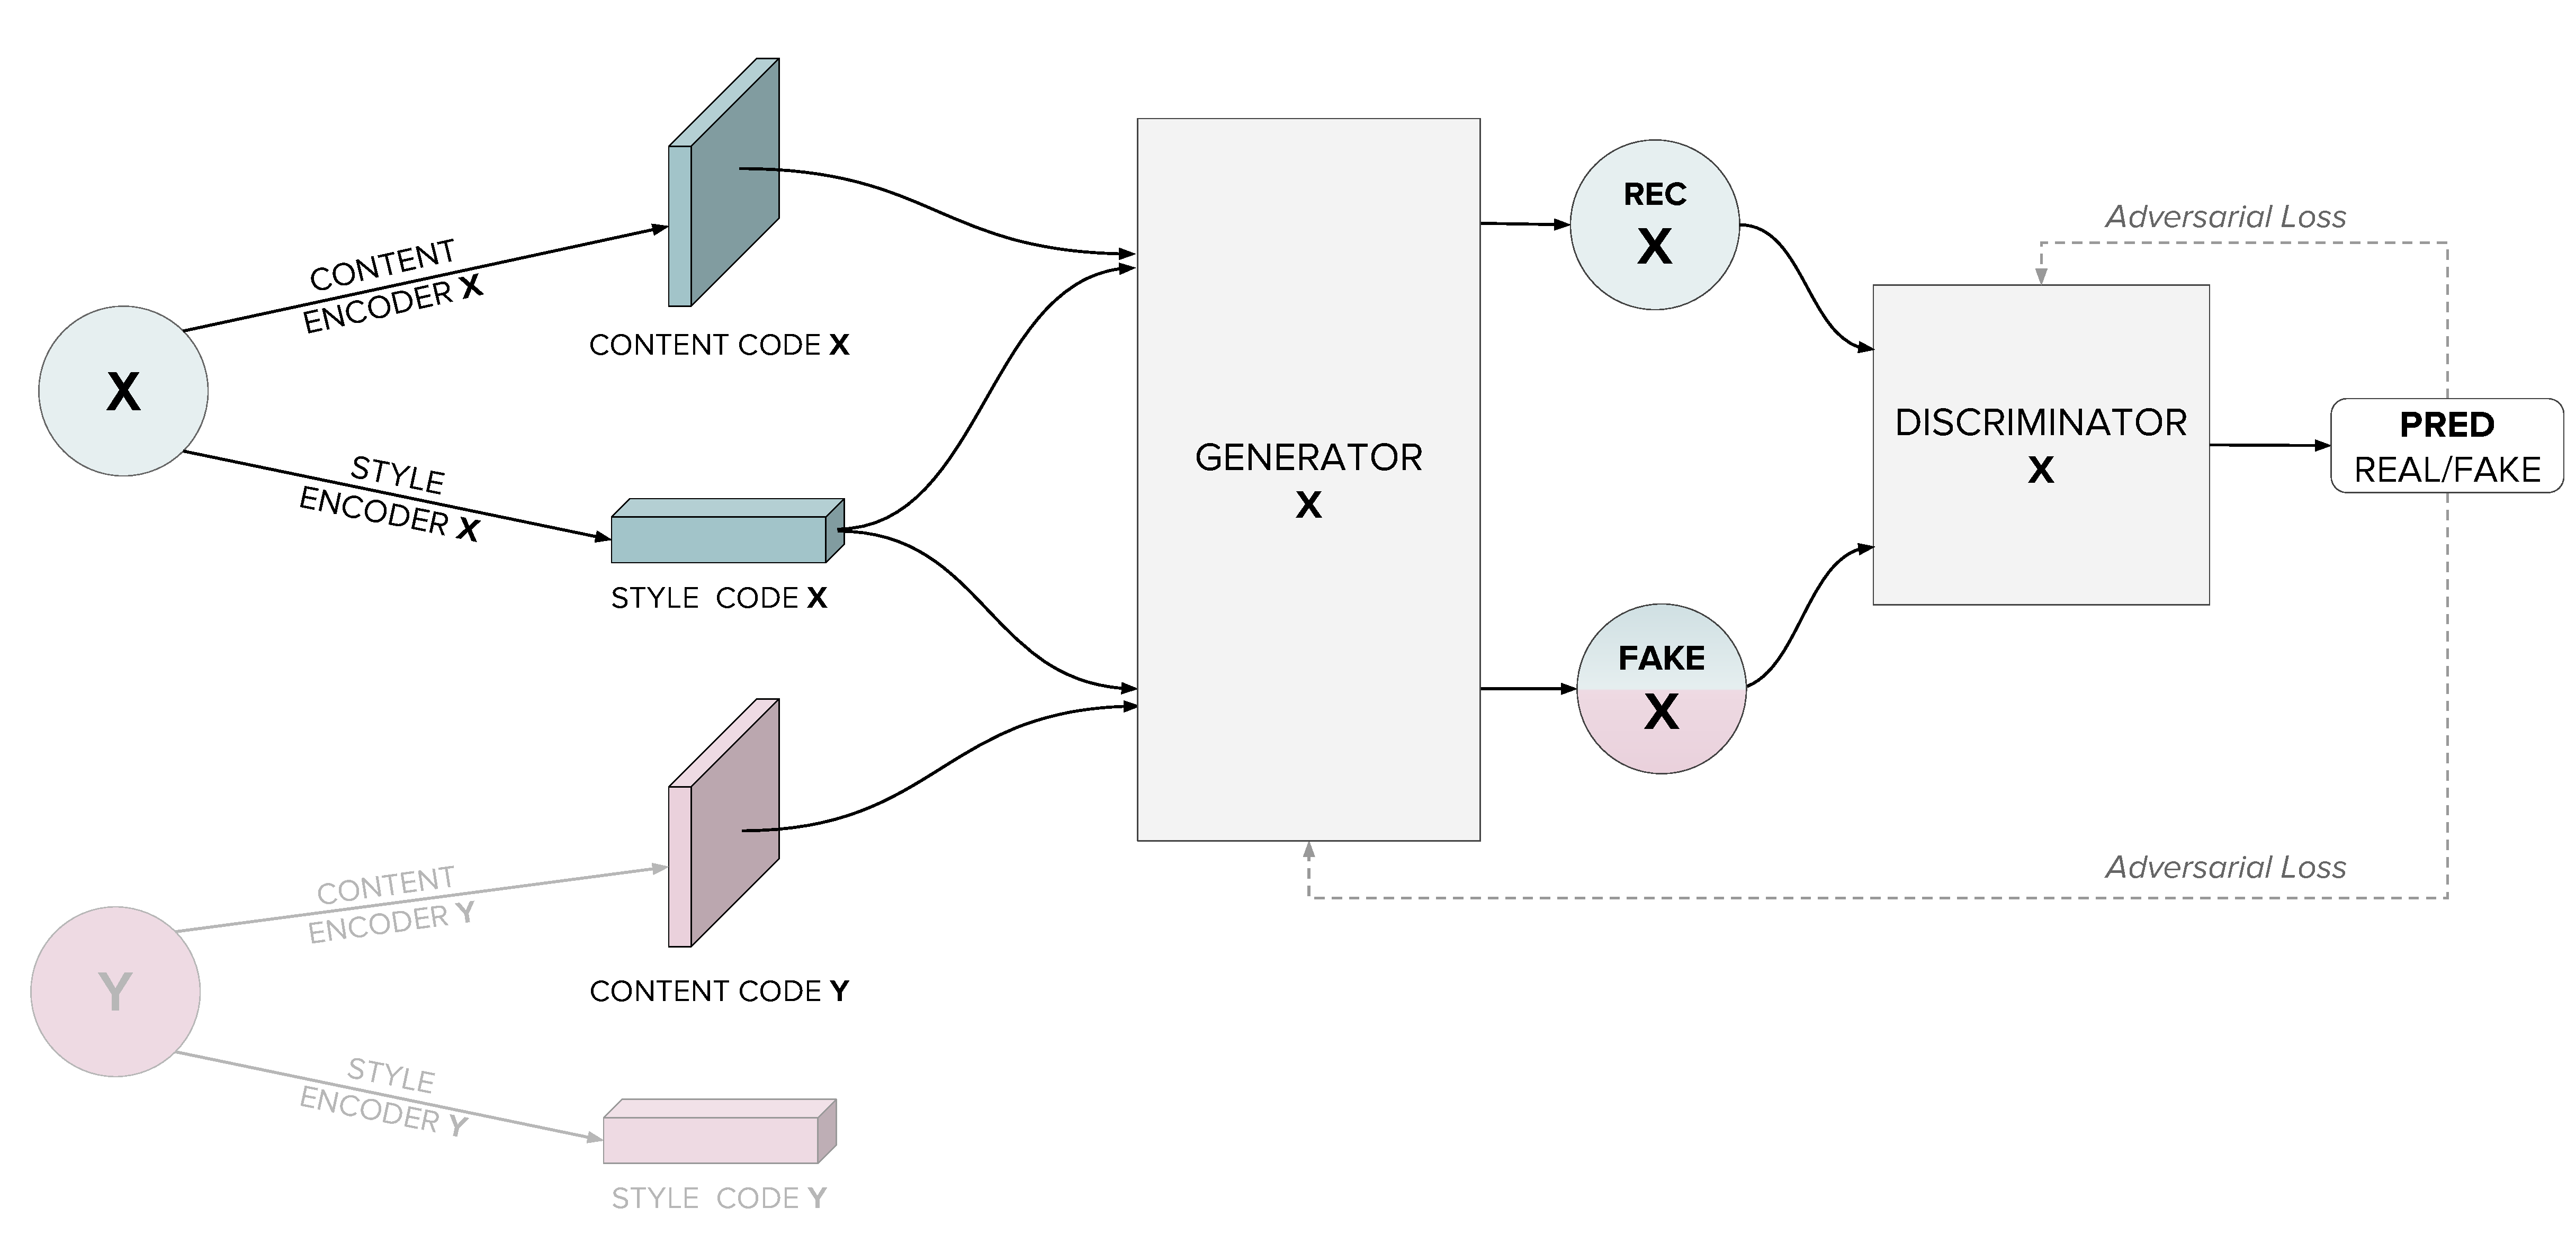
\includegraphics[width=\linewidth]{03_analysis/gans/munit_adv}}
\caption{\label{fig:munit_adv} \textbf{MUNIT cross-domain translation.} The content code of image from domain Y is combined with style from domain X to generate a fake image X. The discriminator decides if the image was translated or comes from the original image domain based on which the adversarial objective is calculated.}
\end{figure}

\paragraph{Adversarial Loss}
In order to enforce the generated output to look realistic, each domain has a discriminator, $D_x$ and $D_y$, which is trained to distinguish if the source of the image is the data distribution of the image domain, or if it was generated by the auto-encoder.
\begin{equation}
\underset{G_x}{\mathrm{min}} \ \underset{D_x}{\mathrm{max}} \ \mathcal{L}^{x}_{adv} = \mathbb{E}_{x}[logD_{x}(x)] + \mathbb{E}_{c_{y}, s_{x}}[log(1 - D_{x}(G_{x}(c_{y}, s_{x})))]
\end{equation}

Figure \ref{fig:munit_adv} shows the adversarial loss for translation from domain $Y$ to domain $X$. The adversarial loss for domain $Y$ is defined similarly.


\paragraph{Training Objective}
The overall training objective, which is trained to be maximized by the discriminators and minimized by the generators and auto-encoders can be modified by $\lambda$, $\lambda_c$, $\lambda_s$, controlling the relative weight of each loss:
\begin{equation}
\underset{G_x, G_y, E_x, E_y}{\mathrm{min}} \ \underset{D_x, D_y}{\mathrm{max}} \ \mathcal{L} = \mathcal{L}^{x}_{adv} + \mathcal{L}^{y}_{adv} + 
\lambda(\mathcal{L}^{x}_{rec} + \mathcal{L}^{y}_{rec}) + 
\lambda_c(\mathcal{L}^{c_x}_{rec} + \mathcal{L}^{c_y}_{rec}) + 
\lambda_s(\mathcal{L}^{s_x}_{rec} + \mathcal{L}^{s_y}_{rec})
\end{equation}


\pagebreak
% ==============================================================
\subsection{Fader Networks}
% ==============================================================
The Fader Networks \cite{lample_fader_2017} is an unsupervised technique of training GANs that, similarly to MUNIT \cite{huang_multimodal_2018}, translates images in latent space instead of pixel space. 

The unique feature of Fader Networks is that the images are modified based on attribute values that are regarded as continuous, e.g: the network can translate a photo of a young person to old person at increasing level of interpolation. Figure \ref{fig:fader_ex} shows example interpolations of different attributes.

Similarly to MUNIT \cite{huang_multimodal_2018}, the model consists of an encoder-decoder architecture, which learns how to translate an input image to its latent representation, and a discriminator to enforce an adversarial approach. In case of Fader Networks the latent representation is a $N$-dimensional vector $z$.

\begin{figure}[h]
\centering
{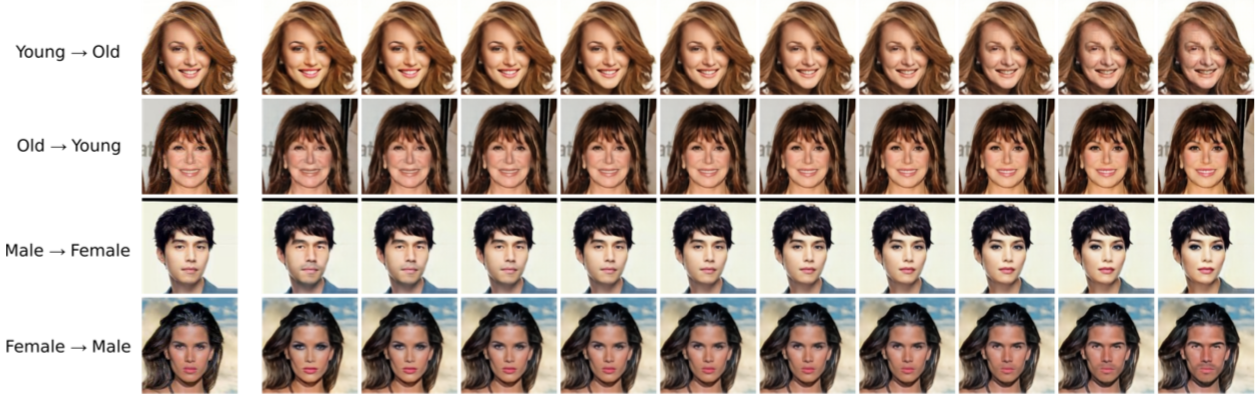
\includegraphics[width=\linewidth]{03_analysis/gans/fader_example}}
\caption{\label{fig:fader_ex} \textbf{FaderNetworks: Interpolations of different attributes.} The original image on the left is translated to the given attribute with increasing intensity from left to right. The outputs of the decoder and discriminator are compared to ground truth and the networks parameters are optimized accordingly. Figure reprinted from \cite{lample_fader_2017}.}
\end{figure}


Given a pair of input image and its corresponding attribute ($x^i \in X, y^i \in Y$), the encoder maps it to its latent representation $z$, $Enc: X \rightarrow \mathbb{R}^N$. The decoder takes a latent vector $z$ and a target attribute $y'$, and translates it to a modified version of the image, $Dec: (\mathbb{R}^N, Y) \rightarrow X$.

The essential feature of this approach is that latent representation of an image is \textit{attribute-invariant}, e.g: an image of the same person young and old should be encoded as the same latent vector. Without this invariance, the decoder would simply learn to ignore the given attribute value. By removing the information about the attributes from the encoded representation, the decoder must consider the attribute in order to reconstruct the image.

However, since paired image training data is not available, the invariance cannot be enforced by adding a simple distance to the loss function, instead it must be learned through an adversarial objective on the latent space. Therefore, the architecture also includes a discriminator network $Dis$, which is trained to predict the attribute value $y$ of an image $x$, given its latent representation $E(x)$.

\begin{figure}[h]
\centering
{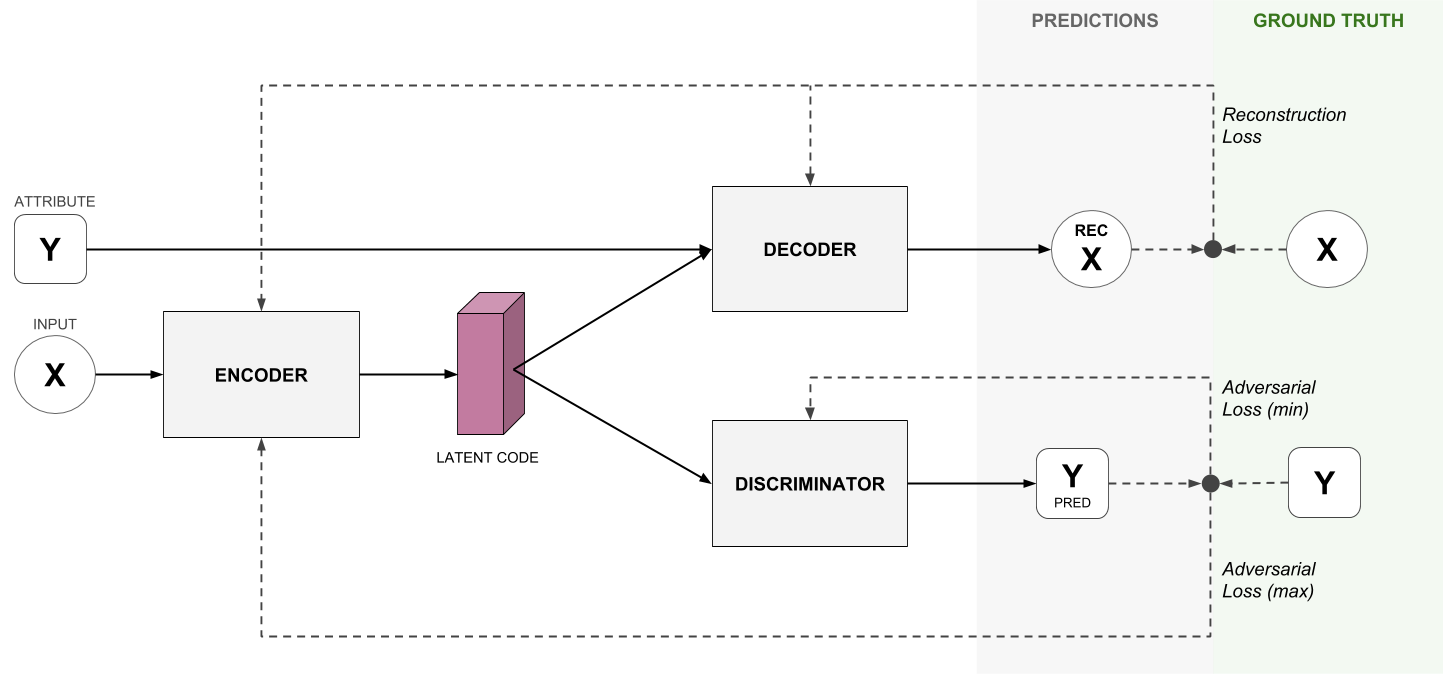
\includegraphics[width=\linewidth]{03_analysis/gans/fader}}
\caption{\label{fig:fader_model} \textbf{FaderNetworks Model.} Given a training pair of input image and attribute value, the image is encoded to a latent code. The decoder learns to reconstruct the image based on its latent code and attribute value, while the discriminator tries to predict the attribute based on the latent code. Figure adapted from \cite{lample_fader_2017}.}
\end{figure}


\paragraph{Reconstruction Loss}
The authors use a \textit{mean squared error} loss (MSE) to optimize the auto-encoder to output images similar to the original inputs. However, they mention that the previously described \textit{PatchGAN} architecture with L1 loss might lead to sharper results.
\begin{equation}
\mathcal{L}_{rec}(Enc,Dec) = \mathbb{E}_{x,y}[||x-Dec(Enc(x),y)||^2_2]
\end{equation}

\paragraph{Adversarial Loss}
The discriminator trains to predict the attributes correctly:
\begin{equation}
\mathcal{L}_{Dis} = \mathbb{E}_{x,y}[log(Dis(y|Enc(x)))],
\end{equation}

while the objective of the encoder is for the decoder to be able to reconstruct the image, and to prevent the discriminator from correctly classifying the attributes:
\begin{equation}
\mathcal{L} = \mathcal{L}_{rec} - \lambda_E \mathbb{E}_{x,y}[log(Dis(1-y|Enc(x)))].
\end{equation}


\pagebreak
% ==============================================================
\section{Image Retrieval Features}
% ==============================================================
I analyzed several available image features that can be used to retrieve images of similar products from the fashion dataset. The most significant differences of the analyzed features are summarized in Table \ref{tab:retrieval_com}. 

The first set of features comes from the Akiwi Application Programming Interface (API) \cite{sonnenberg_akiwi_nodate}, hence an internet connection is necessary to download a feature for a new image. The features are low dimensional and therefore fast to process. The second set of features is created by forwarding the images through a convolutional neural network, which can be done locally. These features are much more high-dimensional - include more information but are also slower to process.

\begin{table}[h]
\centering
\begin{tabular}{@{}lccc@{}}
\toprule
\textbf{Feature Name}                                          & \textbf{Dimensions} & \textbf{Feature Source}    & \textbf{Dataset Used}                                                            \\ \midrule
Akiwi-50                                                       & 50                  & Low-level Features         & -                                                                                \\ \midrule
Akiwi-64                                                       & 64                  & ResNet-200 + Dim. Reduction & ImagNet \\ \midrule
ResNet-152                                                     & 2048                & ResNet-152                 & ImageNet                                                                         \\ \midrule
\begin{tabular}[c]{@{}l@{}}ResNet-152\\ Retrained\end{tabular} & 2048                & ResNet-152                 & \begin{tabular}[c]{@{}c@{}}ImageNet\\ retrained with\\ fashion data\end{tabular} \\ \bottomrule
\end{tabular}
\caption{\label{tab:retrieval_com}\textbf{Comparison of available image features.}}
\end{table}

\subsection{Akiwi}
The Akiwi website \cite{sonnenberg_akiwi_nodate} provides an API, where a user can upload an image file and the API returns a descriptor of the image. This vector can be used as the image feature to compare similarities with other image features.

The API provides various descriptors: the 50-dimensional descriptor is based on low-level features of the image, such as color histogram and edge detection. The 64-dimensional descriptor is produced by the last hidden layer of a ResNet-200 network, normalized and reduced to 64 dimensions \cite{Barthel:2017:VBM:3078971.3079016}.

Figure \ref{fig:akiwi50_feats} shows example of 50-dimensional features visualized as a grayscale color palette of images with smallest and biggest distances.

\begin{figure}[h]
\centering
{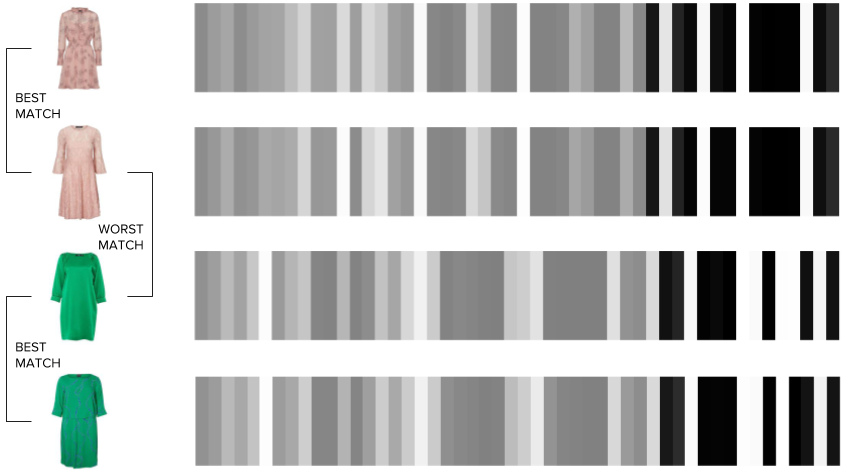
\includegraphics[width=.8\linewidth]{03_analysis/cbir/akiwi50_feats}}
\caption{\label{fig:akiwi50_feats} \textbf{Akiwi 50-dimensional features visualization.} Left column displays the original images. Their respective 50-dimensional feature values are visualized in a grayscale palette.}
\end{figure}


\subsection{ResNet}
Almost every deep learning framework nowadays offers a variety of pre-trained convolutional networks. The deep learning framework PyTorch offers 6 different pre-trained CNN architectures, such as the \textit{VGG Network} \cite{simonyan_very_2014}, \textit{Inception Network} \cite{szegedy_rethinking_2015} or the \textit{ResNet} \cite{he_deep_2015}. 

The networks are pre-trained to classify images from the ImageNet dataset, which contains around 14 million images labeled with 1.000 classes, and has established itself as a reference for testing convolutional architectures. 

Currently, the best scoring pre-trained model offered by PyTorch is the \textit{ResNet152}, which is 152 layers deep and contains so-called \textit{Residual Blocks}. These blocks allow the output of one layer to be added directly to another layer deeper in the network. This technique is useful when training very deep neural networks.

\begin{figure}[h]
\centering
{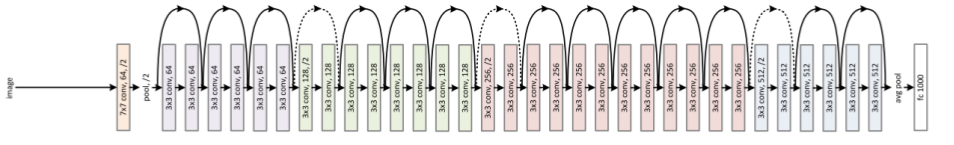
\includegraphics[width=\linewidth]{02_background/CBIR/resnet_arch}}
\caption{\label{fig:resnet34} \textbf{Resnet34 Architecture.} An example of the ResNet architecture with 34 layers. Figure reprinted from \cite{noauthor_resnet-152_nodate}}.
\end{figure}

The extraction of the image feature happens at the last hidden layer of the network, which in case of ResNet152, is a 2048-dimensional layer. For each image, the output of this layer is its unique descriptor, which can be used to compare distances between images.

Since the ResNet152 was trained on a dataset with a big variety of objects, most of the fashion product images likely fall to one category and therefore could have very similar feature vectors, which do not adequately reflect the differences between the products.

However, training such a deep network on a new dataset can be very time consuming and requires the dataset to be quite large. The so-called \textit{Transfer Learning} enables one to use a network trained on a big dataset, such as the ImageNet dataset, and only re-train the last few layers of the network to classify a new dataset. This retrained network, for example to classify the categories of the fashion dataset products, can produce more diverse image descriptors for the given dataset.

\pagebreak
\section{Related Work} \label{sec:related}
Although most of the GANs analyzed in this thesis are general models designed to work with many various datasets, there have also been publications focusing on GANs for fashion-specific tasks, such as modifying a person's outfit or translating image of a person wearing a product to a product image.

Using text-to-image translation, ,,Be Your Own Prada'' \cite{zhu_be_2017} explores the possibility of modifying a product, worn by a person, by describing it with a short description. They first use segmentation to extract the person's pose and then apply a mapping that translates the segment into a new product based on the text description. The model is trained on the DeepFashion dataset, described in Section \ref{sec:data}. The results are shown in Figure \ref{fig:fashiongan}.

\begin{figure}[h]
\centering
{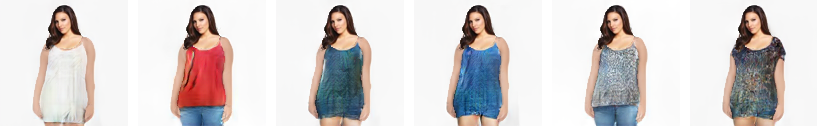
\includegraphics[width=\linewidth]{03_analysis/related/fashiongan}}
\caption{\label{fig:fashiongan} \textbf{FashionGAN.} An original image of a person wearing an outfit is modified based on text description. Figure reprinted from \cite{zhu_be_2017}.}
\end{figure}

A similar approach was also implemented in an image-to-image translation approach by the Conditional Analogy GAN \cite{jetchev_conditional_2017}. Instead of describing the modified outfit with words, the network is provided with an image of a product. The network learns how to swap the current outfit of the person for the given product. The model was trained on dataset provided by Zalando SE \cite{zalando_damenmode_nodate}, a fashion e-commerce retailer, and is not publicly available.

\begin{figure}[h]
\centering
{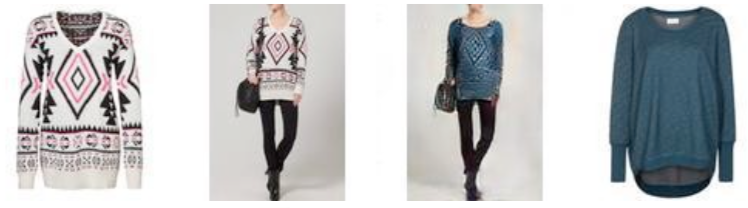
\includegraphics[width=.8\linewidth]{03_analysis/related/cagan}}
\caption{\label{fig:swapgan} \textbf{CAGAN.} Outfit swapping with the Conditional Analogy GAN. On the left is the image training pair and on the right is the generated  image of the input person wearing the target product (on the right). Figure reprinted from \cite{jetchev_conditional_2017}.}
\end{figure}

\pagebreak
Another published image-to-image translation model translates images of people wearing a product to a white-background product image \cite{yoo_pixel-level_2016}. It maps the image from source domain to target domain in pixel-space while preserving the semantic relation between the domains. The results of their research are shown in Figure \ref{fig:pixeldtgan}. Apart from the model, the research also produced a fashion dataset collected from several online fashion stores, consisting of product images and respective images of people wearing the products.

\begin{figure}[h]
\centering
{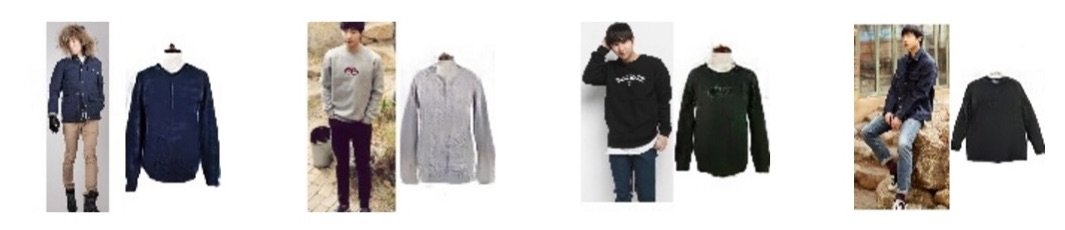
\includegraphics[width=\linewidth]{03_analysis/related/pixeldtgan}}
\caption{\label{fig:pixeldtgan} \textbf{Pixel-Level Domain Transfer.} Results of translation between person domain and product domain with the Pixel-Level Domain Transfer GAn \cite{yoo_pixel-level_2016}. Left: input image, right: generated product image.}
\end{figure}

\pagebreak
% ==============================================================
\chapter{Experiments}
% ==============================================================
The following chapter contains three types of experiments: (1) attribute modification, (2) product to model translation and (3) image retrieval experiments.

The objective of the attribute modification experiments is to test the analyzed generative models on the fashion dataset and evaluate their ability to output a realistic product image with modified attributes. This attribute modification can either effect the shape of the product, such as sleeve length or neckline, or the style of the product, such as its pattern.

The product to model image translation experiment aims to translate the domain of product images to the domain of model images, to expand the possibilities of image retrieval. This section involves data clustering experiments that were necessary to create a supervised dataset for this task.

The image retrieval experiments test different image features to evaluate their retrieval quality both on original product images and also on generated images from previous experiments.

All experiments were performed on the data category of dresses (cca 15.000 images) to reduce the complexity of the experiments and simplify the evaluation process. The experiments were conducted in \textit{Python 3} \cite{noauthor_welcome_nodate}, using the machine learning framework \textit{PyTorch} \cite{noauthor_pytorch_nodate} and several common python packages, including \textit{pandas} \cite{noauthor_python_nodate}, \textit{numpy} \cite{noauthor_numpy_nodate} and \textit{scikit-learn} \cite{noauthor_scikit-learn_nodate}. Since the evaluation of the results is mostly visual, I used \textit{TensorBoard} \cite{noauthor_tensorflows_2018} for visualization of the images and learning curves during training.


% ==============================================================
% ATTRIBUTE MODIFICATIONS
% ==============================================================
\pagebreak
\section{Attribute Modification}
The products in the fashion dataset are described by multiple attributes. These can be modified to allow the user to ,,tailor'' a product according to their taste and trigger a new product search. The experiments in the following section explore the modification of shape and pattern attributes.

These modifications require an unsupervised approach, as there are no image pairs of the same product in both attribute domains, such a sleeveless and a long-sleeved version of the same dress. Moreover, most of the modifications are multi-domain, meaning that the attribute is not binary, but has multiple domains, such as short sleeves, long sleeves or sleeveless. 

\subsection{Data}
Table \ref{tab:data_attr} summarized the attributes modified by the experiments. Since all the experiments were trained using the image category ,,dresses'', I have only chosen to train on attribute values that are well-represented within the category. 

For example, only 12 dress images from the dataset are classified with the attribute value ,,normal length''. This length is usually associated with categories such as blouses and tops in the dataset. Therefore I have excluded this attribute value from the training set. Figures \ref{fig:sleeve_data} - \ref{fig:pattern_data} show example images of each attribute and its values.

\begin{table}[h]
\centering
\begin{tabular}{*{2}{l}{c}}
\hline
Attribute & Possible Values & Attribute Images \\
\hline
Sleeve Length			& long, half, short, sleeveless 		& 13.329\\
Fit			 			& normal, loose, tight 				& 14.661\\
Neckline  				& round, v, wide 					& 10.573\\
Length					& short, knee, long					& 11.362\\
Pattern					& unicolored, floral, print, stripes & 11.165\\
\hline
\end{tabular}
\caption{\label{tab:data_attr}\textbf{Data attributes summary}. Attributes of the fashion dataset and their possible values for category dresses with the respective amounts of images that have one of the possible values assigned.}
\end{table}

\begin{figure}[!h]
\centering
{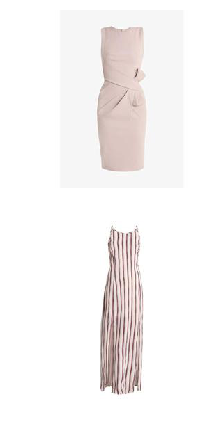
\includegraphics[width=.2\linewidth]{03_analysis/data/sleeves_none}}
{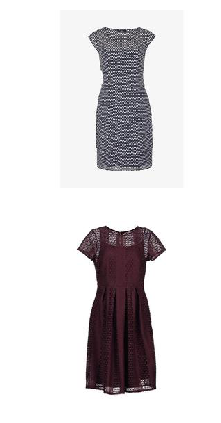
\includegraphics[width=.2\linewidth]{03_analysis/data/sleeves_short}}
{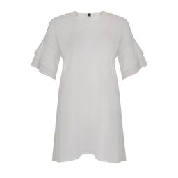
\includegraphics[width=.2\linewidth]{03_analysis/data/sleeves_half}}
{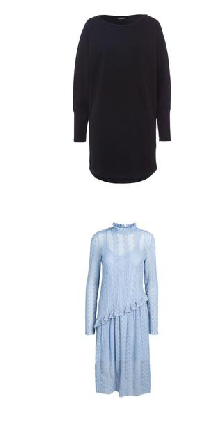
\includegraphics[width=.2\linewidth]{03_analysis/data/sleeves_long}}
\caption{\label{fig:sleeve_data} \textbf{Sleeve-length attribute data.} From left to right: sleeveless, short sleeves, half sleeves and long sleeves.}

{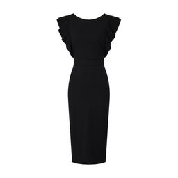
\includegraphics[width=.2\linewidth]{03_analysis/data/fit_tight}}
{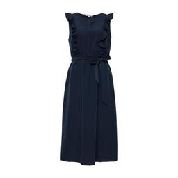
\includegraphics[width=.2\linewidth]{03_analysis/data/fit_normal}}
{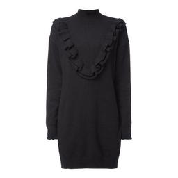
\includegraphics[width=.2\linewidth]{03_analysis/data/fit_loose}}
\caption{\label{fig:fit_data} \textbf{Fit attribute data.} From left to right: tight fit, normal fit and loose fit.}

{\includegraphics[width=.2\linewidth]{03_analysis/data/neckline_v}}
{\includegraphics[width=.2\linewidth]{03_analysis/data/neckline_round}}
{\includegraphics[width=.2\linewidth]{03_analysis/data/neckline_wide}}
\caption{\label{fig:neckline_data} \textbf{Neckline attribute data.} From left to right: v-neck, round and wide neckline.}

{\includegraphics[width=.2\linewidth]{03_analysis/data/length_short}}
{\includegraphics[width=.2\linewidth]{03_analysis/data/length_knee}}
{\includegraphics[width=.2\linewidth]{03_analysis/data/length_long}}
\caption{\label{fig:length_data} \textbf{Length attribute data.} From left to right: short, knee-long and long.}

{\includegraphics[width=.2\linewidth]{03_analysis/data/pattern_unicolors}}
{\includegraphics[width=.2\linewidth]{03_analysis/data/pattern_floral}}
{\includegraphics[width=.2\linewidth]{03_analysis/data/pattern_stripes}}
{\includegraphics[width=.2\linewidth]{03_analysis/data/pattern_print}}
\caption{\label{fig:pattern_data} \textbf{Pattern attribute data.} From left to right: unicolors, floral, stripes and print.}
\end{figure}

\pagebreak
\subsection{Shape Translation}
Since the shape translation is an unsupervised and multi-domain task, StarGAN is the most suitable network from the evaluated models. I used the official StarGAN implementation written in PyTorch to train the models: \linebreak \hyperlink{https://github.com/sonynka/StarGAN}{github.com/sonynka/StarGAN}. The exact architecture is displayed in Figure \ref{fig:stargan_arch}.

%TODO change batch size and image size if experimnets succesffull
I used batch size of 8 throughout the experiments and image size of $128 \times 128$ pixels. I was not able to train bigger image sizes due to lack of GPU memory in the laboratory servers. Each experiment was trained for 40 epochs, which in practice translated to around 5 training hours on a Tesla M40 12GB GPU. The original source code for StarGAN updates the discriminator weights five times for one generator update. 

Theoretically, StarGAN should be able to learn one generator mapping for all the attributes and their values. However, to reduce the complexity of the model, I decided to train one generator per each attribute, namely: sleeve length, length, fit and neckline.

\vspace{0.5cm}
\begin{figure}[h]
\centering
\subcaptionbox{Discriminator}{\includegraphics[width=\linewidth]{04_experiments/stargan/dis_arch}}\vspace{.5cm}
\subcaptionbox{Generator}{\includegraphics[width=\linewidth]{04_experiments/stargan/gen_arch}}
\caption{\label{fig:stargan_arch} \textbf{Experiment StarGAN Architecture.} The architecture of the trained  discriminator and generator. CONV denotes a convolutional layer, IN denotes instance normalization, LRELU denotes leaky relu with slope 0.2.}
\end{figure}

The original model without modifications yielded good results on the fashion dataset, but the outputs contained checkerboard-like artifacts - a quite common effect when upsampling images with transposed convolution, or ,,deconvolution'' \cite{odena2016deconvolution}.

\begin{figure}[h]
\centering
{\includegraphics[width=.5\linewidth]{04_experiments/stargan/checkerboard}}
\caption{\label{fig:stargan_checkerboard} \textbf{Checkerboard Artifacts.} Left: Output of the original StarGAN model with visible checkerboard-like artifacts. Right: Output of a modified model which uses bilinear interpolation instead of transposed convolution to resize the image.}
\end{figure}

To avoid this issue, I inserted an upsampling layer before every ,,deconvolution''. This layer uses bilinear interpolation to double the size of the image. The ,,deconvolution'' layer, that is applied after upsampling, keeps the size of the image and only reduces the number of channels. This results in smoother outputs with less artifacts, as shown in Figure \ref{fig:stargan_checkerboard}.

I also discovered an instability of the model color understanding - in the first few training iterations, sometimes the generator learns to map the original color to a different one, such as shown in Figure \ref{fig:stargan_color}. If this happens early on in the training, the network is not able to recover and keeps outputting flipped colors.

The reconstruction loss does not penalize this issue, since the generator reconstructs the image back to its original color. I therefore added a L1 distance term to the loss function, which measures the distance between the generated and the real image in order to prevent color changes.

\begin{figure}[h]
\centering
{\includegraphics[width=.7\linewidth]{04_experiments/stargan/color_flip}}
\caption{\label{fig:stargan_color} \textbf{Color-flipped StarGAN outputs.} The generator learns to map images to different domains to a different color.}
\end{figure}

\pagebreak
Figure \ref{fig:sleeves_results} shows the results of sleeve length modification. StarGAN learns the mapping relatively early on in the training, however, the network generator struggles with dresses that have a strong pattern, or are very light colored.

\begin{figure}[h]
\centering
{\includegraphics[width=.7\linewidth]{04_experiments/stargan/sleeve_results}}
\caption{\label{fig:sleeves_results} \textbf{Sleeve-Length Modiciation Results.} The left column shown the input image, while the rest of the columns show the generated outputs with sleeve-length modifications, such as: sleeveless, short sleeves, half sleeves and long sleeves. Displayed input images are from the test set.}
\end{figure}

To solve this issue, I experimented with modeling the generator as a U-Net, discussed in section \ref{sec:pix2pix}, instead of the original ResNet architecture described in the paper \cite{choi_stargan_2017}. However, the U-Net generator failed to start learning the domain mappings.

I also tried hyperparameter modifications, such as lowering the generator's learning rate, or changing the relative weights of each loss. None of these experiments have improved the results.

\pagebreak
Translation of sleeve length seemed to be the easiest for the network to learn. The same network trained on other attribute translations, such as neckline and fit, outputs less realistic images, that contain a lot of artifacts. This may be due to the fact, that these attributes are much more subtle than sleeve length - which is quite obvious shape change. Figure \ref{fig:neckline_results} shows results of neckline and fit translation.

\begin{figure}[!h]
\centering
\subcaptionbox{Neckline Translation Results}{
{\includegraphics[width=.45\linewidth]{04_experiments/stargan/neckline_results}}}
\subcaptionbox{Fit Translation Results}{
{\includegraphics[width=.45\linewidth]{04_experiments/stargan/fit_results}}}
\caption{\label{fig:neckline_results} \textbf{Neckline and Fit Modification Results.} The left column shown the input image, while the rest of the columns show the generated outputs. \textbf{(a)} Neckline modifications: round, v-neck and wide neckline. \textbf{(b)} Fit modifications: tight, normal, loose fit.}
\end{figure}

The attribute length was the hardest to train and the network did not find a proper mapping for the attribute. Therefore I have decided to exclude this attribute from the shape modification possibilities.

\pagebreak
\subsection{Style Translation}
In this experiment, the goal of the translation is for the content of the image - the product shape - to be maintained and only the style to be modified. these experiments can be understood as a style transfer. The most fitting models for this task are therefore those that allow a latent representation of the image, in order to separate the content from the style. I experimented with 3 models for this task: FaderNetworks, MUNIT and CycleGAN>

\subsubsection{FaderNetworks}
The FaderNetworks are unique among the evaluated models in their ability to gradually interpolate between two domains. In the example of style transfer, the user can decide, for example, how of a floral pattern the dress should have.

I have trained the network to translate the floral and stripes pattern of the images, while using the original set-up of the official PyTorch implementation: \linebreak \hyperlink{https://github.com/sonynka/FaderNetworks}{github.com/sonynka/FaderNetworks}.

As seen in Figure \ref{fig:fader_results}, the network trained to translate unicolor domain to striped-pattern domain is able to represent the original image without the pattern. However, the applying of the pattern leads to a ,,burn'' effect of not only the product but also the background of the image.

\begin{figure}[h]
\centering
{\includegraphics[width=\linewidth]{04_experiments/fader}}
\caption{\label{fig:fader_results} \textbf{FaderNetworks Pattern Translation Results.} The left-most image is the original input. Next to it is its attribute-invariant representation. Next, the stripes pattern is gradually applied to the image.}
\end{figure}

Since changes to the hyperparameters of the network did not improve the results, I decided to abandon this experiment and try pattern translation with a different network.

\pagebreak
\subsubsection{MUNIT}
Ideally, the output of style translation should be multi-modal - one unicolored dress should have more than one possible floral-patterned versions and vice versa. MUNIT is the only network from the evaluated networks that models a multi-modal approach. It also provides a ,,guided'' style transfer, so that the user can ,,guide'' the style of a dress in one domain to style of a specific dress in another domain.

I used the official PyTorch implementation, published by NVidia: \linebreak\hyperlink{https://github.com/sonynka/MUNIT}{github.com/sonynka/MUNIT} - with changes to adapt it to the dataset and logging structure. I used batch size of one to avoid problems with insufficient GPU memory and the default training parameters. The network was trained for 50.000 iterations, which took around 12 hours on the previously mentioned GPU.

\begin{figure}[h]
\centering
{\includegraphics[width=\linewidth]{04_experiments/munit/munit_results}}
\caption{\label{fig:munit_results} \textbf{MUNIT Pattern Translation Results.} Domain A represents floral-patterned dresses, domain B represents unicolored dresses. Guided style translation translates the input image A to style of input image B and vice versa. Random style translation chooses a random style from each respective domain to apply to the input images. The displayed images are from the test set.}
\end{figure}

Figure \ref{fig:munit_results} shows the results of experiments translating the floral pattern to unicolor domain and vice versa. The network learns the content encoding correctly and the shape of the dresses is maintained in the translation. It also learns to map floral dresses to unicolor dresses. However, it fails to find the right encoding for the floral style. As shown in the Guided Style example of Figure \ref{fig:munit_results}, the generated image takes the color of the input but not the floral pattern.

I experimented with increasing the dimension of the style encoding from the original 8 dimensions to 16 and 32, as well as tuning hyperparameters of the network such as learning rate and the relative weight of each term in the loss function. However, none of the experiments have resulted in a reasonable interpretation of the floral style.

\subsubsection{CycleGAN}
Since experiments using MUNIT did not yield the desired result, I experimented with the more simple model of CycleGAN, which does not offer either the multi-modality nor the ,,guided'' style transfer functionality of MUNIT. Instead it trains the translation in pixel-space.

I used the official PyTorch implementation by the authors of the paper: \linebreak \hyperlink{https://github.com/sonynka/pytorch-CycleGAN-and-pix2pix}{github.com/sonynka/pytorch-CycleGAN-and-pix2pix}. The model uses a ResNet architecture for the generator and a simple convolutional network for discriminator, as shown in Figure \ref{fig:cyclegan_arch}.

\begin{figure}[h]
\centering
\subcaptionbox{Discriminator}{\includegraphics[width=.8\linewidth]{04_experiments/cyclegan/cycle_discriminator}}\vspace{.5cm}
\subcaptionbox{Generator}{\includegraphics[width=\linewidth]{04_experiments/cyclegan/cycle_generator}}
\caption{\label{fig:cyclegan_arch} \textbf{Experiment CycleGAN Architecture.} The architecture of the trained  discriminator and generator. CONV denotes a convolutional layer, IN denotes instance normalization, LRELU denotes leaky relu with slope 0.2.}
\end{figure}

The model was trained with batch size 8 and learning rate 0.0001. The image size was 128 $\times$ 128 pixels. I trained one generator for each of the patterns in the dataset: floral, stripes and print, each of them paired with unicolored domain. The models were trained for 150 epochs (cca 12 hours on the used GPU). 

Results of floral pattern translation are shown in Figure \ref{fig:cycle_floral_results}. It learns the mapping of both translation directions while keeping the shape of the dresses as well. Some of the outputs contain minor artifacts around the dress.

\begin{figure}[h]
\centering
\subcaptionbox{Floral to Unicolors}{\includegraphics[width=.45\linewidth]{04_experiments/cyclegan/floral_from}}
\subcaptionbox{Unicolors to Floral}{\includegraphics[width=.45\linewidth]{04_experiments/cyclegan/floral_to}}
\caption{\label{fig:cycle_floral_results} \textbf{CycleGAN Floral Pattern Translation Results.} Results of the translation between floral and unicolor domains in both directions on test set images.}
\end{figure}

Although CycleGAN does not produce multi-modal outputs, some multi-modality can be introduced by using generators from various epochs towards the end of the training. At this stage of training the pattern translation is already trained well and the changes in the output are more influenced by the current batch of training images. 

As shown in Figure \ref{fig:cycle_floral_multimodal}, the outputs from epochs 120, 130 and 150 are all realistic but vary in the colorfulness and scale of the floral pattern. This approach can be used to introduce some multi-modality. However, this approach can be only used when mapping from unicolored domain, since the other directions does not vary the output based on the epoch that much.

\begin{figure}[h]
\centering
{\includegraphics[width=\linewidth]{04_experiments/cyclegan/floral_multimodal}}
\caption{\label{fig:cycle_floral_multimodal} \textbf{CycleGAN Multi-Modality.} Results of the translation between floral and unicolor domains on test images. Left image is the input image, the images on the right are outputs of epoch 150, 130 and 120 respectively.}
\end{figure}

Results for translating stripes pattern are shown in Figures \ref{fig:cycle_stripes_results}. The outputs contain more artifacts and are not as realistic as floral pattern - less training data for this domain can be the cause of worse results. I also experimented with the print pattern, however, the prints in the input images are so diverse - ranging from a simple logo through a full paisley print, that the network had difficulties to recognize the mapping.

\begin{figure}[h]
\centering
\subcaptionbox{Stripes to Unicolors}{\includegraphics[width=.45\linewidth]{04_experiments/cyclegan/stripes_from}}
\subcaptionbox{Unicolors to Stripes}{\includegraphics[width=.45\linewidth]{04_experiments/cyclegan/stripes_to}}
\caption{\label{fig:cycle_stripes_results} \textbf{CycleGAN Stripes Pattern Translation Results.} Results of the translation between stripes and unicolor domains in both directions on test set images.}
\end{figure}

% ==============================================================
% PRODUCTS TO MODLES
% ==============================================================
\pagebreak
\section{Products to Models Translation}
Some online fashion retailers provide product images that are taken on white background without a person modeling the product. However, there are also many images online, coming from other retail platforms, social media and blogs of people wearing a certain product, without a corresponding product image. The goal of this experiment was to translate a product image to an image of a person wearing that product, in order to expand the search possibilities.

I first experimented with the MUNIT network - an unsupervised approach, translating between the domain of all product images and the domain of all model images. This approach has not yielded the desired results, since the output was too diverse and it failed to represent the input product.

Therefore I have decided to train a network in a supervised manner, such that it learns to map an image of a specific product to an image of a model wearing that specific product. This task required a dataset consisting of image pairs, which I created using a clustering algorithm.

\subsection{Data Clustering}
As mentioned in Section \ref{sec:data}, each scraped product has a variable amount of images displaying people modeling the given product. The average amount of images per product is 4, and based on manual screening of the dataset, a product usually has these types of model images: full-body model front-facing, full-body model back-facing, zoom to part of body were product is worn and large zoom on detail.

In order to create a dataset of image pairs for supervised training, each product must have exactly one corresponding model image. I chose the model image that most of the products should have - where the model is facing the camera and the full body is captured. 

However, there is no clear order or pattern from which to deduce the pose of the model based on the name of the image or its position in the list of images. Since there are more than 60.000 model images only for category dresses, manual selection of the best image for each product would be too time consuming.

To identify the best image for each product, I used the following approach:
\begin{enumerate}
	\item \textbf{Image Processing}: Highlight relevant features for the selection, such as contours, while suppressing irrelevant features, such as color.
	\item \textbf{Clustering}: Cluster features and experiment with amount of clusters.
	\item \textbf{Select Best Cluster}: Visualize clusters and manually select the best cluster center.
	\item \textbf{Select Best Image}: For each product, select the image with the smallest distance to the best cluster center.
\end{enumerate}


For clustering, I used the \textit{K-Means Clustering} algorithm \cite{noauthor_k-means_2018}, which creates $k$ clusters and assigns each data point to the nearest cluster center. The \textit{scikit-learn} library offers a fast implementation of the algorithm \cite{noauthor_sklearn.cluster.kmeans_nodate}.

\subsubsection{Grayscale Clustering}
For the initial experiment, I have converted the model images to grayscale, in order to separate the person from the background regardless of the color of the product they are wearing. 

In order to reduce the dimensionality and speed up the algorithm, I resized the images to $64\times64$ pixels. The total number of model images is $63.103$, which means the clustering algorithm was fed with an array of size $63103\times64\times64$.

%\begin{figure}[h]
%\centering
%{\includegraphics[width=.8\linewidth]{04_experiments/clustering/grayscale}}
%\caption{\label{fig:cluster_gray} \textbf{Cluster centers with grayscale features.} The left most column displays the cluster centers and the rest columns display random images from the dataset that are assigned to the respective cluster based on their grayscale feature vector.}
%\end{figure}

%Figure \ref{fig:cluster_gray} shows the results of K-Means clustering with 4 cluster centers. Although the second cluster center groups the desired image type, it does so only for dark-colored dresses. As one can see from the results, the fourth cluster center tends to group all images with light-colored dresses, in all poses. 

However, the clustering algorithm tented to group model images not only by pose, but also by color. All light-colored dresses were usually grouped to one cluster, regardless of the pose in the image. Therefore grayscale features do not fit the requirement for the clustering process to disregard color as a feature.


\subsubsection{Edges}
In order to avoid the problem of separating dark and light colors into different clusters, I used \textit{Canny Edge Detection} algorithm to highlight the pose of the model in the model image. This feature only considers the contours of the object in the image and is invariant to the color of the dress.

\begin{figure}[h]
\centering
{\includegraphics[width=\linewidth]{04_experiments/clustering/edges_data}}
\caption{\label{fig:cluster_edges_data} \textbf{Canny Edge Detection for model images.} Each left image shows original image and right image shows the corresponding edges produced with Canny Edge detection algorithm.}
\end{figure}

This feature, however, is sensitive to edges created on images with darker background. All model images were resized to a uniform size of $256\times256$ as part of the data collection process, by extending the short side of the image with white color. The edge detection algorithm recognizes this transition on images with darker gray background, such as shown in Figure \ref{fig:cluster_edges_data}. 

The clustering experiments using these feature were therefore affected by this detection and tended to group images with darker backgrounds together, regardless of the model pose. Therefore, in all further experiments, the images have center-cropped width of 116 pixels.

Overall, clustering with edges did not prove to be effective, as the edges are very thin and therefore the measured distance between two images, which are quite similar, but a little bit shifted, would be very big. The detection is also sensitive to patterns in the dresses, as seen in Figure \ref{fig:cluster_edges_data}.

\subsubsection{Threshold Mask}
To avoid the difficulties with thin edges, I used a thresholding technique to fill the person's contour with white color and background with black. By applying Gaussian blur to the images before the threshold mask, this feature is invariant to the pattern or style of the dress. Figure \ref{fig:cluster_outline_data} shows the steps applied to each image to get a binary threshold mask.

\begin{figure}[h]
\centering
{\includegraphics[width=\linewidth]{04_experiments/clustering/outlines_data}}
\caption{\label{fig:cluster_outline_data} \textbf{Threshold Mask for model images.} Starting from left is the original image, converted to grayscale, applied Gaussian blur, binary threshold, and the image masked with binary threshold.}
\end{figure}

This feature selection has proven to be the most effective for \textit{K-Means} algorithm with 3 cluster centers. First column of Figure \ref{fig:cluster_outline} shows the three cluster centers: the first groups full-body photographs, second groups zoomed images of upper-body and the last one groups detail images. 

\begin{figure}[h]
\centering
{\includegraphics[width=\linewidth]{04_experiments/clustering/outlines_clusters}}
\caption{\label{fig:cluster_outline} \textbf{Cluster centers with threshold mask.} The rows A-C show 3 cluster centers created by \textit{K-Means Clustering} algorithm with threshold mask features of images. Each column $1-6$ shows one product and the image that is closest to the respective cluster center.}
\end{figure}

Each row of Figure \ref{fig:cluster_outline} shows the image that is the closest to the respective cluster center for the given product 1-6. The products can have more model images, that are not displayed because they are not the best match for any of the cluster centers, as well as one model image can be best match for more than one cluster center. 

We can observe that products $1-4$ are grouped according to expectations. Product $5$ is problematic, because the dress is lighter than the background and therefore its features do not match the cluster centers as expected. Product $6$ is an example of an outlier product, where there are no model images available and instead only a product image is provided.

Figure \ref{fig:cluster_outline_distances} shows all available images for product 1 sorted based on their respective distances to cluster center \textbf{A}. The first picture is therefore the best match for the cluster center.

\begin{figure}[h]
\centering
{\includegraphics[width=\linewidth]{04_experiments/clustering/outlines_distances}}
\caption{\label{fig:cluster_outline_distances} \textbf{Product images distances to cluster center A.} Images are sorted by the distances towards cluster center A from Figure \ref{fig:cluster_outline}.}
\end{figure}

Based on these results, I selected cluster center \textbf{A} from Figure \ref{fig:cluster_outline} as the best and for each product chose the image which is closest to that center. Although there are some outliers in the results, the network working with this data should be able to learn to ignore them.

% --------------------------------------------------------------------------------------------
\pagebreak
\subsection{Training}
Pix2Pix \cite{isola_image--image_2016} is the only network from the evaluated models that translates images in a supervised matter. I have modified the official PyTorch implementation of the paper \cite{noauthor_junyanz/pytorch-cyclegan-and-pix2pix_nodate}, in order to work with the fashion data structure: \hyperlink{https://github.com/sonynka/pytorch-CycleGAN-and-pix2pix}{github.com/sonynka/pytorch-CycleGAN-and-pix2pix}.

Figure \ref{fig:pix2pix_arch} describes the used architecture of the network. In all experiments, I have used image size 256 and batch size 8. The learning rate starts at 0.0002 and is decreased gradually towards 0 throughout the training. Both networks are optimized using Adam optimizer. The experiments were trained for 40 epochs - around 20 hours on Tesla M40 12GB GPU.

\begin{figure}[h]
\centering
\subcaptionbox{Discriminator}{\includegraphics[height=1.5cm]{04_experiments/pix2pix/dis_arch}}\vspace{.5cm}
\subcaptionbox{Generator}{\includegraphics[width=\linewidth]{04_experiments/pix2pix/gen_arch}}
\caption{\label{fig:pix2pix_arch} \textbf{Pix2Pix Architecture.} The architecture of the trained  discriminator and generator. CONV denotes a convolutional layer with kernel size 4 and stride 2 unless indicated otherwise, BN denotes batch normalization, LRELU denotes leaky relu with slope 0.2 and DO denotes drop out with rate 50\%. Figure adapted from \cite{hesse_image--image_2017}.}
\end{figure}

Training with the original set-up of the network resulted in a common GAN failure, discussed in Section \ref{sec:gan_diff}: the discriminator learns to distinguish the source of an image confidently too fast, resulting in the generator not having opportunity to improve. This behavior can be observed in Figure \ref{fig:pix2pix_losses}a, where the generator loss keeps growing throughout the training, while discriminator loss is minimized early on.

To avoid this issue, I added some noise to the labels to confuse the discriminator and give the generator and advantage in the training. In my implementation, the real labels are chosen randomly in each iteration from a value range between 0.7 to 1.2 and fake labels from a value range between 0.0 and 0.3 \cite{chintala_starter_2018}. I also experimented with flipping the labels for the discriminator every once in a while, so that real images are described as fake and vice versa. As shown in Figure \ref{fig:pix2pix_losses}b, by disadvantaging the discriminator, both losses get stabilized.

\begin{figure}[t]
\centering
\subcaptionbox{Original Model}{\includegraphics[width=.48\linewidth]{04_experiments/pix2pix/loss_original}}
\subcaptionbox{Label Noise}{\includegraphics[width=.48\linewidth]{04_experiments/pix2pix/loss_soft_labels}}
\caption{\label{fig:pix2pix_losses} \textbf{Pix2Pix Adversarial Loss.} Adversarial loss of the discriminator and the generator, a) with the original pix2pix set-up, b) with adding noise to discriminator. For visualization purposes, the curves are smoothed, such as described in \cite{noauthor_tensorflows_2018}. The real loss values are shown in the background.}
\end{figure}

Although the learning curves can provide an insight into the staibility of the training, there is no objective method to correlate the losses to whether the results look realistic - the network's outputs need to be evaluated mostly visually \cite{preserve_knowledge_how_nodate}. 

Figure \ref{fig:pix2pix_results} shows the generated samples from the test set for 3 different models. The different training parameters for each model are summarized in Table \ref{tab:pix2pix_exp}. 

\begin{table}[h]
\centering
\begin{tabular}{@{}lccc@{}}
\toprule
                 & Original Model & Noisy Labels      & Lower Learning Rate \\ \midrule
Batch Size       & 8              & 8                 & 8                   \\
Epochs Trained   & 140            & 140               & 140                 \\
Learning Rate    & 0.0002         & 0.0002            & 0.0001              \\
Real Label Value & 1.0            & 0.7 - 1.3         & 0.7 - 1.3           \\
Fake Label Value & 0.0            & 0.0 - 0.3         & 0.0 - 0.3           \\
Flip Labels    & No             & 10/100 Iterations & 5/100 Iterations    \\ \bottomrule
\end{tabular}
\caption{\label{tab:pix2pix_exp} \textbf{Pix2Pix Experiments Training Parameters.}}
\end{table}

\pagebreak
The original model produces visually inconsistent results: some generated outputs look realistic enough, as product 1 and 2, while others seem to fail. For example, for products 4 and 5, the generator produces almost identical output with a slight change of color.

We can observe that the model which uses noisy labels, where the discriminator is not as strong, does not have these issues and overall produces more stable results. The same model trained with a lower learning rate is better at capturing the textures of the input image.

\begin{figure}[!h]
\centering
{\includegraphics[width=.8\linewidth]{04_experiments/pix2pix/results}}
\caption{\label{fig:pix2pix_results} \textbf{Generated test set images of pix2pix model with different modifications.} The first two columns show the input image and the corresponding target image. The outputs come from the original implementation of the model, model with added label noise to confuse the discriminator and a model with learning rate 0.0001 respectively.}
\end{figure}

% ==============================================================
% IMAGE RETRIEVAL
% ==============================================================
\pagebreak
\section{Image Retrieval}

\subsection{Dataset Images}
In this part of the image features comparison, I have used the original product images from the dataset as input to retrieve the most similar images. Figure \ref{fig:search_pink} illustrates the strengths and weaknesses of the tested feature vectors. 

Akiwi50 retrieves images that have similar color palettes but different shapes, while Akiwi64 does the opposite: it retrieves similarly shaped products regardless of their color. Although the two features combined together return more sensible results, given that the input dress is not very unique in the dataset, the results are still not very accurate. 

The ResNet features are quite similar, however in both ResNet and ResNet retrained there are outliers of images that do not fit color-wise. The combination of the original ResNet feature with the color-focused Akiwi50 prevents this issue and returns the most similar images.

\begin{figure}[h]
\centering
{\includegraphics[width=.48\linewidth]{04_experiments/retrieval/akiwi_pink}}\hspace{0.2cm}
{\includegraphics[width=.48\linewidth]{04_experiments/retrieval/resnet_pink}}
\caption{\label{fig:search_pink} \textbf{Image retrieval results with tested feature vectors.} The left shows the Akiwi Features, the right one shows ResNet Features. Each row shows the input image in the left column and the best 5 matches based on L2 distance between the respective feature vectors. The number under each image represents its distance to the input}.
\end{figure}

\pagebreak
I also evaluated the retrieved results based on the metric used - L1 distance and L2 distance. Figure \ref{fig:search_weights} compares retrieved results  using these two distances for different features and their combinations. As shown in the last two rows of Figure \ref{fig:search_weights}, displaying the combination of ResNet features and Akiwi50 features in different ratios, L1 distance supports the retrieval of more color-like images, while L2 distance retrieves more shape-like products. 

\begin{figure}[!h]
\centering
\subcaptionbox{L1 Distance}{
{\includegraphics[width=.48\linewidth]{04_experiments/retrieval/resnet_l1}}}\hspace{0.2cm}
\subcaptionbox{L2 Distance}{
{\includegraphics[width=.48\linewidth]{04_experiments/retrieval/resnet_l2}}}
\caption{\label{fig:search_weights} \textbf{Image retrieval results with different combinations of ResNet and Akiwi50 features.} Displaying the results for two different input images, the first row shows an equal ratio, second row shows 1:2 ratio and third row shows 1:3 ratio when combining ResNet and Akiwi50 features respectively.}.
\end{figure}

\subsection{Synthesized Images}
Although the experiments on real images from the dataset reveled the strenghts and weaknesses of the tested features, the feature should be able to correctly retrieve similar images based on a generated input. This input can contain artifacts and overall not be as high-quality as the original images. 

\begin{figure}[h]
\centering
\subcaptionbox{Floral to Unicolors}{
{\includegraphics[width=.48\linewidth]{04_experiments/retrieval/generated/floral_from}}}\vspace{0.3cm}
\subcaptionbox{Unicolors to Floral}{
{\includegraphics[width=.48\linewidth]{04_experiments/retrieval/generated/floral_to}}}
\caption{\label{fig:search_weights} \textbf{Image retrieval results with generated patterns.} In each figure (a) and (b), the top left image is the original input and underneath it is its translated version to or from floral domain respectively. The rest of the images are most similar images. Retrieved images are based on Resnet+Akiwi50 (1:2) feature and L1 distance.}
\end{figure}

\begin{figure}[h]
\centering
{\includegraphics[width=\linewidth]{04_experiments/retrieval/generated/pix2pix_retrieval}}
\caption{\label{fig:search_weights} \textbf{Image retrieval results with generated models.} The image on the left is the input product image. Top row shows the retrieved the images for the original model image and the bottom row shows the retrieved images for the generated model image. Retrieved images are based on Resnet+Akiwi50 (1:2) feature and L1 distance.}
\end{figure}




\chapter{Results}
The final model generates new product images based on user-specified modifications and uses the generated images to trigger a search of existing products that are visually similar. The objective of this tool is to enable users to search through large amounts of fashion items faster and more interactively, regardless of what types of filter options are available.

As illustrated in Figure \ref{fig:pipeline}, a dress image from the dataset is passed to a \textit{Product Synthesis} module, where the dress shape and pattern are modified based on user input. This generated image is passed through another network, \textit{Model Synthesis}, to generate an image of a person wearing the fake dress. Both the generated product image and the generated model image are then passed to the \textit{Product Search} and \textit{Model Search} modules respectively. The feature vectors of the generated images are calculated, and compared to features of original images from the dataset. Based on this comparison, the most similar images are retrieved from the dataset.

\vspace{0.5cm}
\begin{figure}[h]
\centering
{\includegraphics[width=\linewidth]{05_results/pipeline}}
\caption{\label{fig:pipeline} \textbf{Fashion GAN Search Pipeline.}}
\end{figure}

The project is written in Python and the GAN search application is provided as a \textit{Jupyter Notebook}. The product modification and search can be controlled by the user via text input. The source code of the project can also be found on GitHub: \linebreak \hyperlink{https://github.com/sonynka/fashion\_gan}{github.com/sonynka/fashion\_gan}. For more information about the source code, please see the Documentation in Appendix \ref{app:doc}.

\section{Synthesis}
Based on the results of the experiments, the final model uses three out of the five evaluated image-to-image translation models: StarGAN for shape modifications, CycleGAN for pattern modifications and Pix2Pix for product-to-model translation. Each of the used GANs was chosen for its specific task in the model based on its characteristics. Hereby, the focus was not to generate a highly realistic new garment, but to generate realistic enough output to retrieve similar existing products from the dataset.

Surprisingly, the common characteristics of the used networks is pixel-space translation, as opposed to encoding the images into a latent representation, such as the evaluated MUNIT network and FaderNetworks. The latent representation models offer more sophisticated translation options, such as multi-modality, which also makes them more complex and, based on my experience, harder to train and interpret. The pixel-space networks are easier to evaluate and overall yielded more stable outputs on the fashion dataset.

\paragraph{Shape Modification}
The StarGAN network is used for modifying the shape attribute due to its ability of multi-domain training, therefore reducing the amount of generator networks that had to be trained. The final model was trained using the official PyTorch implementation: \hyperlink{https://github.com/sonynka/StarGAN}{github.com/sonynka/StarGAN}. In order to prevent checkerboard artifacts in the output, I added a bilinear upsampling layer before every deconvolution. I also added an L1 term to the overal loss of the generator, which measures the L1 distance between the generated image and the original image, to prevent the generator from changing the products color.

The quality of the outputs vary from attribute to attribute - sleeve length modification outputs sharp and clean images, while modification of neckline and fit, resulted in less realistic output with more artifacts. The cause is vague training data: sleeve length categories are visually very well distinguishable, while the differences between fits of the dresses are hard to categorize, and neckline attribute is often indicated only by a slight transition of color (Figure \ref{fig:problem_data}).

\begin{figure}[h]
\centering
\subcaptionbox{Round neckline vs. V-neckline}{
{\includegraphics[width=.23\linewidth]{05_results/neckline_round}}
{\includegraphics[width=.23\linewidth]{05_results/neckline_v}}
}
\vspace{0.2cm}
\subcaptionbox{Tight fit vs. loose fit}{
{\includegraphics[width=.23\linewidth]{05_results/fit_tight}}
{\includegraphics[width=.23\linewidth]{05_results/fit_loose}}
}
\caption{\label{fig:problem_data} \textbf{Examples of similar images from different categories.} \textbf{(a)} Dresses with different neckline categories. The difference is hard to distinguish due to the dark color of the dresses. \textbf{(b)} Two fit categories that are supposed to be opposite, but look similar.}
\end{figure}

StarGAN also struggles with reconstructing detailed structures in the products, such as patterns or other decorative elements. This can be due to the bottleneck architecture of the generator through which the original input must pass, and therefore low-level details that both input and output share, get lost. One of the solutions of this problem is to use a U-Net architecture (Section \ref{sec:pix2pix}), however, in my experiments, U-Net generator failed to learn the translation.

\paragraph{Pattern Modification}
The loss of patterns when translating an attribute with StarGAN, can be partly recovered by applying a new pattern to the product using the trained CycleGAN. CycleGAN is used for pattern modification due to its ,,style transfer'' nature - the network keeps the content of the image while changing its style.

The CycleGAN was trained to translate unicolor images to floral or stripes pattern, and vice versa, resulting in a total of 4 trained generators. The network was not able to train with the pattern ,,print'' that is available in the dataset. This was also due to the fact that the pattern of the images in this category is very variable, raging from a small brand logo to a full animal print of the garment.

The final model was trained with the original open-source PyTorch implementation available at: \linebreak \hyperlink{https://github.com/sonynka/pytorch-CycleGAN-and-pix2pix}{github.com/sonynka/pytorch-CycleGAN-and-pix2pix}. 

While floral translation works well with most of images, the stripes modification output is not as stable. One of the reasons could be the distortion of very fine stripes in the images.  Figure \ref{fig:stripes_retrieval} demonstrates image retrieval with an existing striped image and a generated striped image. Even though the generated striped image is one of the best results of the stripe-translation, the pattern is not clearly recognized by the feature and the retrieval results are mixed with other patterns.

\begin{figure}[h]
\centering
{\includegraphics[width=\linewidth]{05_results/stripes_orig_results}}
{\includegraphics[width=\linewidth]{05_results/stripes_gen_results}}
\caption{\label{fig:stripes_retrieval} \textbf{Fashion GAN Search Results.} Top left image is the original test image, images in the left column underneath are modified versions of the original image. For each image in the left column retrieved images are shown in the respective row. Images were retrieved with Resnet+Akiwi50 feature and L1 distance.}
\end{figure}

One of the major drawbacks of CycleGAN is the lack of a multi-modal output. The floral pattern in the dataset can range from very detailed white flowers to large colorful flower patterns. CycleGAN however, is not able to capture this variety in the output. I introduced some multi-modality in the final model by sending the input image through three snapshots of the CycleGAN model. These snapshots were created after different epochs towards the end of the training and display some variation in the pattern, especially when applied to dark-colored dresses. However, this multi-modality is only limited and mostly visible on dark-colored dresses. The snapshot that the image is sent through at each modification is chosen randomly. I only introduced this approach for floral pattern, as the variation in different snapshots of the stripes model was not obvious.

%
%Initially, the model was designed so that one can change the attributes of one product multiple times, e.g: first shorten the sleeves and then round the neckline. However, using a synthesized image as an input for a consecutive synthesis can magnify artifacts and blurriness of the result. To avoid this behaviour, the final application allows the user to change one attribute of the dress, trigger a new image search, select a similar existing product, and then modify further.


%\begin{figure}[h]
%\centering
%\subcaptionbox{Input $\rightarrow$ Pattern $\rightarrow$ Shape}{
%{\includegraphics[width=.48\linewidth]{05_results/consecutive_mod1}}}
%\subcaptionbox{Input $\rightarrow$ Shape $\rightarrow$ Pattern}{
%{\includegraphics[width=.48\linewidth]{05_results/consecutive_mod2}}}
%\caption{\label{fig:consecutive_mod} \textbf{Differences between Consecutive Modifications.} Shape modification can result in loss of pattern details (a), therefore it is better, to first modify shapes and then patterns (b).}
%\end{figure}

\paragraph{Product-to-Model Translation}
After each modification, the generated image is sent through the Pix2Pix network, which produces an image of a person wearing the generated product. This generated model image is supposed to help find more similar products, that are photographed on a person.

Since products in the original dataset have more than one picture of a person wearing the product assigned, this task first required a clustering of the data in order to create a 1:1 paired image dataset of product and model image. The data was clustered with a K-Means algorithm using a black-and-white threshold mask of the images as input, in order to choose the model image for each product where the person's full-body is photographed.

The final Pix2Pix model was trained using the official open-source PyTorch implementation: \hyperlink{https://github.com/sonynka/pytorch-CycleGAN-and-pix2pix}{github.com/sonynka/pytorch-CycleGAN-and-pix2pix}. The original set-up has resulted in a common failure of GANs, where the discriminator is too strong and does not leave generator the opportunity to improve. Therefore I implemented several strategies to confuse the discriminator, described in detail in the Experiments section.

The outputs of the Pix2Pix network are not realistic - modeling a person's body and face is too complex for the given networks. The generated images only capture basic characteristics of the products, such as its color or length. More detailed characteristics, such as shape or pattern get lost in the translation. Good retrieval results can usually be achieved only on simple uni-colored silhouettes that are well represented within the dataset. Therefore the usefulness of this feature for the image retrieval can be debated. A more reasonable approach might be the one from some of the related research mentioned in Section \ref{sec:related}, where an image of a person is first segmented and then only the fashion garment segment is generated, rather than the whole person.

\begin{figure}[h]
\centering
{\includegraphics[width=\linewidth]{05_results/model_retrieval}}
\caption{\label{fig:model_retrieval} \textbf{Generated Model retrieval.} Left image is original product input, next to it the generated model image. The rest of the images are retrieved as most similar to the generated image.}
\end{figure}

\section{Retrieval}
Based on the experiments with different feature vectors, the final model uses a combination of 2048-dimensional ResNet feature and 50-dimensional low-level Akiwi feature, in the ratio of 1:2. The features are combined based on L1 distance. The ResNet feature is extracted from the last hidden layer of ResNet152 pretrained on ImageNet dataset. The 50-dimensional feature is calculated using the Akiwi API \cite{sonnenberg_akiwi_nodate}, and influences the output to include more color-like images.

However, the results of the retrieval can only be evaluated subjectively. For example, the use of L2 distance instead of L1, retrieves products that are more similar in shape and less similar in color, which some users might prefer.

\begin{figure}[h]
\centering
{\includegraphics[width=.8\linewidth]{05_results/gan_search}}
\caption{\label{fig:pipeline_images} \textbf{Fashion GAN Search Results.} Top left image is the original test image, images in the left column underneath are modified versions of the original image. For each image in the left column retrieved images are shown in the respective row.}
\end{figure}

The retrieval features are relatively robust when comparing features of generated output against original images. However the features can be effected by too many artifacts in the outputs.  Although initially the model was designed so that one can change the attributes of one product multiple times (e.g: first shorten the sleeves and then round the neckline), using a synthesized image as an input for a consecutive synthesis can magnify artifacts and blurriness of the result. Therefore the final application allows the user to change one attribute of the dress, trigger a new image search, select a similar existing product, and then modify further.



\chapter{Conclusion and outlook}
The outcome of this thesis is a model that can generate new fashion product images based on user input. These generated images are then used as input for an image retrieval system in order to retrieve most similar existing products from the dataset. The synthesized fashion products are not highly realistic, but they suffice as input in order to influence the retrieval of the images. The developed tool could be further improved and used to browse fashion datasets, for example in online stores or fashion product aggregator sites, regardless of what search and filter options are available.

The success of this type of project is dependent on the available dataset. The modification options that are available, as well as the quality and resolution of synthesized images and therefore the retrieval features, can be improved by providing higher-quality and quantity data. Due to the lack of available open-source fashion datasets, that contain products photographed on a white background, the dataset used for this thesis was scraped from various online fashion stores. The heterogeneity of the sources means that the descriptions of the products, such as sleeve length or fit, are difficult to unify. This leads to vaguely-defined categories that are hard to distinguish and therefore hard to train on. The dataset is also hard to extend, as the scraped websites can change their structure and data.

Therefore, for further development of this project, more attention should be focused on acquiring a cleaner dataset with well-defined and represented categories, that is also easily extensible in order to stay up-to-date with the latest fashion trends.

\appendix

\newpage
\pagenumbering{roman}
\addcontentsline{toc}{chapter}{Bibliography}
\bibliographystyle{unsrtnat}
\renewcommand{\refname}{Bibliography}
\bibliography{zotero}
\clearpage

% ========================================================================
\pagestyle{plain}
\addcontentsline{toc}{chapter}{Statutory Declaration}
\chapter*{Statutory Declaration}
I assure that this thesis is a result of my personal work and that no other than the indicated aids have been used for its completion. Furthermore I assure that all quotations and statements that have been inferred literally or in a general manner from published or unpublished writings are marked as such. Beyond this I assure that the work has not been used, neither completely nor in parts, to pass any previous examination.

\vspace{2cm}
\noindent
Berlin, 29 September 2018
\hfill
Sona Pecenakova
\clearpage

\chapter{Documentation} \label{app:doc}

\end{document}
